\documentclass[twoside,11pt]{article}

\PassOptionsToPackage{hyperfootnotes=false}{hyperref}
\usepackage[abbrvbib]{jmlr2e}
\usepackage{times}
\hypersetup{hidelinks,
  pdftitle={Scale Sensitivity of Regional Uncertainty in Physics-Informed Neural Networks:
    A Full-Network Gauss--Newton Study},
  pdfauthor={Soumyadip Mal and Nagaiah Chamakuri}}
% Packages jmlr2e does not provide.
\usepackage{amsmath, mathtools}
\usepackage{booktabs, multirow, array}
\usepackage{enumitem}
\usepackage{lastpage}
\usepackage{placeins}

\let\pinnorigunderscore\_
\renewcommand{\_}{\pinnorigunderscore\allowbreak}
\emergencystretch=1.5em

\newcommand{\Rrms}{R_{\sigma}^{\mathrm{rms}}}
\newcommand{\achratio}{\widehat{R}_{\sigma}}

\newcommand{\rmratio}{\widetilde{R}_{\sigma}}
\newcommand{\ratiogap}{\rho}
\newcommand{\meanwidthgap}{\rho_{\mathrm{mw}}}
\newcommand{\meanZ}{\overline{Z}}
\newcommand{\Rtar}{R_{\mathrm{tar}}}
\newcommand{\sh}{\mathrm{s}}
\newcommand{\bk}{\mathrm{b}}
\newcommand{\Pisl}{\Pi_{\mathrm{sl}}}
\newcommand{\Pist}{\Pi_{\mathrm{st}}}
\DeclareMathOperator{\spn}{span}

\jmlrheading{}{2026}{1-\pageref{LastPage}}{}{}{}{Soumyadip Mal and Nagaiah Chamakuri}

% Running head: must be 50 characters or fewer.
\ShortHeadings{Scale Sensitivity of Regional PINN Uncertainty}{Mal and Chamakuri}
\firstpageno{1}


\begin{document}

\title{Scale Sensitivity of Regional Uncertainty in Physics-Informed Neural Networks:
       A Full-Network Gauss--Newton Study}

\author{\name Soumyadip Mal \email soumya24@iisertvm.ac.in \\
        \name Nagaiah Chamakuri\thanks{Corresponding author.} \email nagaiah.chamakuri@iisertvm.ac.in \\
        \addr School of Mathematics\\
        Indian Institute of Science Education and Research Thiruvananthapuram\\
        Vithura, Trivandrum, Keralam 695551, India}

\editor{}

\maketitle
\setcounter{bottomnumber}{2}
\raggedbottom

\begin{abstract}%
Physics-informed neural networks (PINNs) can be accurate on average yet inaccurate
in thin layers and at moving interfaces. Useful uncertainty estimates should
reflect these regional differences. We ask whether post-hoc Gaussian uncertainty
from Gauss--Newton curvature, a linearised Laplace approach, places uncertainty
where numerical errors occur. Its covariance depends on a prior scale and a
common residual-noise scale. We evaluate full-network covariances for $17$
Burgers and Allen--Cahn runs with two
architectures, comparing reference-defined sharp and bulk regions. Allocation is
strongly scale-dependent. For the trained prediction, five of eight Burgers--MLP
runs have identified precisions matching sharp-to-bulk uncertainty and error
ratios; these span more than four orders of magnitude. No match is found for three
runs in the tested range. Neither training-based scale choices nor the tested
predictive centres reliably calibrate both regions. Even at the matching points,
a reference-informed oracle calibrating bulk coverage to $68\%$ yields only
$30.3$--$55.7\%$ sharp coverage for the trained prediction. Reference-based readout
refits reveal features capable of representing sharp structures. Spectral analysis
explains how the scales redistribute uncertainty across curvature modes, with key
bounds machine-checked in Lean~4. Matching regional uncertainty ratios therefore
does not ensure calibrated intervals: allocation and coverage must be assessed
separately.
\end{abstract}

\begin{keywords}
physics-informed neural networks, uncertainty quantification, Gauss--Newton covariance,
calibration, spectral analysis
\end{keywords}

\section{Introduction}\label{sec:intro}

Physics-informed neural networks (PINNs) approximate the solution of a partial
differential equation (PDE) by minimising residuals of the governing equation,
initial and boundary conditions, and available observations at sampled training
points \citep{raissi2019pinns}. Competing loss terms and differential-operator
conditioning can impede optimisation
\citep{wang2021understanding,rathore2024challenges}; collocation strategies can
also fail to propagate initial and boundary information into the interior
\citep{daw2023r3}. Converting a small sampled residual loss into a solution-error
bound requires suitable stability and sampling conditions
\citep{mishra2023generalization}. The remaining
error can be highly non-uniform: a network may approximate the smooth bulk
accurately while retaining substantial error near a thin layer or moving
interface. Domain-averaged diagnostics can conceal this concentration.

Uncertainty estimates could help identify these locally unreliable predictions,
but their interpretation depends on what they describe. In scientific machine
learning, uncertainty may arise from noisy observations, limited information about
model parameters, or numerical approximation error in the computed solution
\citep{psaros2023uq}. These sources need not concentrate in the same parts of
the domain. In particular, uncertainty under a residual-based training model
need not track numerical approximation error.
Bayesian PINNs combine physical constraints with a probabilistic model of noisy
observations and propagate the resulting parameter uncertainty to the solution
\citep{yang2021bpinns}. Deep ensembles use variation between independently trained
predictors \citep{lakshminarayanan2017ensembles}. Whether this predictive spread
tracks numerical approximation error must be assessed rather than assumed.

Local Gaussian methods construct uncertainty around a single trained network
\citep{daxberger2021laplace}. A Laplace approximation uses the Hessian of the
negative log-posterior at a posterior mode. For a Gaussian residual likelihood,
the Gauss--Newton approximation replaces the negative log-likelihood Hessian by
the noise-scaled residual Jacobian Gram matrix, omitting residual second-derivative
terms. With a Gaussian
prior, the resulting covariance is also the exact posterior covariance of the
linearised (affine) residual model at the chosen checkpoint. Linearising the output
propagates this parameter covariance to predictive variances
\citep{immer2021linearized}. In the related setting of neural operators, LUNO
uses model linearisation to propagate Gaussian weight uncertainty into a
function-valued Gaussian process \citep{magnani2025linearization}. This
operator-learning setting differs from our fixed-solution residual model.
\citet{kristiadi2021learnable} show that uncertainty geometry can change while
point predictions remain fixed, motivating a separate assessment of covariance
allocation.

The prior precision and residual-noise variance determine the relative strength
of prior regularisation and residual constraints. Marginal likelihood, or
evidence, integrates the likelihood over the prior and provides a training-based
criterion for selecting these scales \citep{immer2021evidence}.
\citet{antoran2022evidence} account for the difference between a trained
checkpoint and the affine posterior optimum using a fixed network linearisation.
PINN applications already include eikonal travel-time inversion for hypocentre
localisation with diagonal-Fisher curvature \citep{izzatullah2022hypopinn}, and
the heat, wave and Burgers equations with full-Hessian Laplace inference and
evidence-based selection of prior strength and residual weights
\citep{graczyk2026bayesian}. Our regional audit freezes the checkpoint and
relative residual weights, leaving that joint training and hyperparameter-selection
procedure outside the comparison.

Complementary approaches connect uncertainty more directly to numerical accuracy.
Error-Aware B-PINNs incorporate numerical discrepancy into predictive uncertainty
\citep{graf2022erroraware}; solution-error bounds can set spatially varying
likelihood widths in a second Bayesian fitting stage \citep{flores2025errorbounds}.
Calibration assesses whether interval coverage agrees with its nominal level.
Physics-informed conformal prediction uses PDE residuals as nonconformity scores
to calibrate coverage in residual space
without labelled solutions \citep{gopakumar2025calibrated}. Conformal calibration
of PINN predictions uses labelled solution values, with local quantiles allowing
spatially adaptive bands \citep{yu2026conformal}. Marginal coverage guarantees,
under their stated assumptions, do not by themselves ensure coverage conditional
on membership in a sharp region. Section~\ref{sec:discussion} illustrates this
distinction with a split-conformal example. Our contribution is a controlled
regional audit of a full-network residual Gaussian: scale and centre comparisons,
reference feature refits and spectral analysis separate covariance allocation
from interval coverage. Our audit asks how useful this covariance is for describing
deterministic solution error under the specified likelihood.

We study two nonlinear parabolic problems: viscous Burgers, where nonlinear
transport competes with diffusion and produces a thin layer, and Allen--Cahn,
a reaction--diffusion equation with moving phase interfaces. The two architectures
are an independent-feature multilayer perceptron (MLP) and its random-Fourier-feature
variant. For each fixed trained network, we use the Gaussian posterior of the
frozen affine residual and output model. Write $z=(x,t)$ for a space--time point,
$u_\theta(z)$ for the trained prediction and $g(z)=\nabla_\theta u_\theta(z)$ for
its parameter sensitivity. Let $J$ be the Jacobian of the weighted training
residuals and $F=J^\top J$.

\begin{samepage}
For isotropic prior precision $\alpha>0$ and common
weighted-residual variance $v>0$, the parameter covariance $\Sigma$ and latent
predictive variance $\sigma^2$ are
\begin{equation*}
 \Sigma=v(F+\gamma I)^{-1},\qquad
 \sigma^2(z)=g(z)^\top\Sigma g(z),\qquad \gamma=\alpha v.
\end{equation*}
\end{samepage}
The prior variance is $1/\alpha$ in each parameter direction, and $\sigma(z)$ is
the predictive standard deviation, without an added output-noise term. The common
variance is applied after the fixed block weights. At fixed effective
precision $\gamma$, the affine predictive centres and uncertainty contrasts are
unchanged, while widths scale as $\sqrt v$. Our plug-in baseline uses $v=1$ and
$\alpha_0=1/\langle\theta^2\rangle$, with the mean square taken over all trainable
weights and biases; this rule is not evidence maximisation. All these parameters
enter the covariance. The Fourier frequencies are fixed embedding constants and
are excluded from $\theta$ (Section~\ref{sec:setting}).

Reference-gradient percentiles define the sharp and bulk regions, separated by
a transition region (Definition~\ref{def:regions}). We compare sharp-to-bulk
root-mean-square (RMS) uncertainty and error contrasts. Equal contrasts mean equal
relative concentration, without determining absolute width or within-region
coverage. The predictive centre is the prediction around which intervals are
drawn. Because the prior is absent during training, the affine posterior mean
can differ from the trained output. Comparing priors centred at zero and at
$\theta$ isolates shrinkage towards zero from the likelihood correction. We also
evaluate the shifted nonlinear network as a forward diagnostic with covariance
frozen at $\theta$. Reference solutions determine the regions and run admission,
provide evaluation errors, and enter the explicitly reference-informed oracle and feature-refit
diagnostics. At a specified checkpoint and scales, the covariance is formed from
training residuals and network sensitivities.

All $17$ admitted runs have a baseline allocation deficit: uncertainty is less
concentrated in the sharp region than the error (Table~\ref{tab:ceiling};
Figure~\ref{fig:burgers-slice}). This relative deficit coexists with substantial
regional overcoverage. The training-based scale choices change both properties:
with trained centres, the conditional noise maximum-likelihood estimate
under-covers both regions in all eight Burgers--MLP seeds, while finite-grid
evidence selections frequently
reach the lower noise boundary and can be numerically sensitive. Five
Burgers--MLP seeds have identified contrast-matching precisions spanning more
than four orders of magnitude; three retain the deficit throughout the sampled
range.

Centring the prior at the checkpoint retains the baseline deficit in all $17$
runs. Relative to the trained prediction, its affine mean improves full-grid
accuracy in $15/17$ runs at the conditional noise-MLE scales, without calibrating both
regions; nonlinear evaluation instead worsens bulk error in all $17$.
Even an oracle that matches trained-centre
RMS contrasts and calibrates bulk coverage to $68\%$ gives only
$30.3$--$55.7\%$ sharp coverage at the five identified Burgers--MLP matching
points. Thus regional allocation and interval coverage are separate properties.
Readout refits assess feature expressivity, while spectral analysis explains the
scale dependence of covariance allocation.

\begin{figure}[t]
\centering
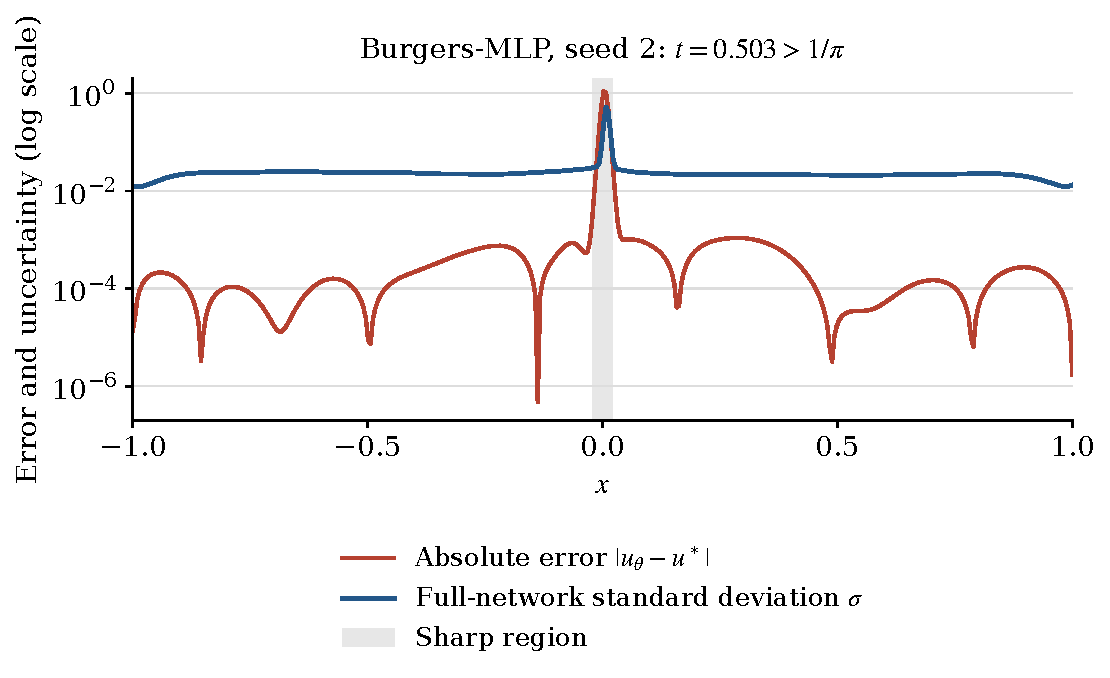
\includegraphics[width=.94\textwidth]{figures/burgers_error_uncertainty_slice.pdf}
\caption{Burgers--MLP seed $2$: absolute error and full-network baseline standard
deviation at $t=0.503$, the stored slice nearest $t=0.5$, after breaking time $1/\pi$.
The logarithmic scale is shared without rescaling; shading marks the global sharp
region of Definition~\ref{def:regions}. Error is more concentrated near the layer.
Here $|e|>\sigma$ near its centre; this is seed-specific, with post-formation calibration
varying across seeds (Table~\ref{tab:temporal}). Full-grid contrasts are in
Table~\ref{tab:ceiling}.}
\label{fig:burgers-slice}
\end{figure}

\begin{samepage}
\emph{Contributions.}
\begin{itemize}
\item \emph{Scale sensitivity and regional coverage (Section~\ref{sec:ceiling}).}
The tested scales and centres do not reliably calibrate both regions. The baseline
deficit survives the alternative prior centre, and direct evaluation at refined
contrast-matching precisions confirms that RMS agreement is insufficient after
bulk calibration.
\item \emph{Reference feature expressivity (Section~\ref{sec:offmanifold}).}
Using reference values to refit the final linear layer leaves below $4\%$ of the trained
sharp-region error energy on held-out time blocks in $16/17$ runs. This tests feature
expressivity independently of residual-only coefficient selection.
\item \emph{Spectral weighting (Section~\ref{sec:theory}).}
A ratio of weighted spectral sums explains scale dependence. In the canonical runs,
covariance weighting amplifies modest regional differences in total tangent norms.
Two-subspace bounds constrain contrast but are too wide to certify the measured
baseline deficit. Lean~4 verifies the spectral bounds and conditional scale limits,
prior-centre bounds and coverage envelopes; reported run counts remain numerical.
\end{itemize}
\end{samepage}

\emph{Empirical scope.}
All eight attempted Burgers--MLP seeds are admitted. Burgers--Fourier,
Allen--Cahn--MLP and Allen--Cahn--Fourier each have three admitted runs selected
by the error criterion in Section~\ref{sec:setting} and are exploratory.
Attempted counts and rejected settings remain explicit. The results concern the
specified training-weighted residual metric and reference-based partition.

\section{Setting and Definitions}\label{sec:setting}

We specify the equations, admission rule and frozen affine model before comparing
regional uncertainty under changes of scale and predictive centre.

\emph{Equations and trained networks.}
On $(x,t)\in[-1,1]\times[0,1]$, the viscous Burgers equation is
\[
 u_t+u u_x=\nu u_{xx},\qquad \nu=0.01/\pi,\qquad
 u(x,0)=-\sin(\pi x),\qquad u(\pm1,t)=0.
\]
The positive-viscosity solution remains smooth and develops a thin layer near $x=0$.
We use the inviscid breaking time $1/\pi$ to define pre- and post-formation windows.
The Allen--Cahn equation is
\[
 u_t=\varepsilon^2u_{xx}+5(u-u^3),\qquad \varepsilon^2=10^{-4},\qquad
 u(x,0)=x^2\cos(\pi x),
\]
with periodic boundaries and interfaces of width $O(\varepsilon)$ between phases
$u\approx\pm1$. A contextual linear control is recorded in Appendix~\ref{app:training};
it is outside the nonlinear scale study.

The independent-feature MLP has $20$ spatial and $20$ temporal sub-networks feeding
a fusion head, with $P=196{,}009$ parameters. Replacing its input layer by random
Fourier features gives $P=275{,}369$ at bandwidth $\mathrm{FS}$
\citep{tancik2020fourier}. The parameter vector $\theta\in\mathbb R^P$ contains
all trainable network weights and biases. The sampled Fourier frequencies are
held fixed throughout training and uncertainty analysis and are excluded from
$\theta$. Both networks are trained in float64 by Adam
\citep{kingma2015adam} followed by Levenberg--Marquardt
\citep{levenberg1944,marquardt1963}. Evaluation uses a uniform $400\times200$ grid ($80{,}000$
points); the residual Jacobian has $N=6400$ rows: $5000$ collocation, $1000$
initial-condition and $400$ boundary rows. Training locations are sampled uniformly
once per seed and held fixed; seeds jointly vary these locations, network
initialisation and, for Fourier models, embedding frequencies. The Burgers reference uses the Cole--Hopf
solution with $80$-node Gauss--Hermite quadrature, agreeing with independent
log-space quadrature to $4.5\times10^{-14}$. The Allen--Cahn reference uses
fourth-order exponential time differencing with $512$ modes and $1000$ steps
\citep{kassam2005etdrk4}; refinement to $2048$ modes changes the canonical contrast
by less than $0.1\%$. Appendix~\ref{app:training} records the training details.
Unless a seed count is stated, numerical illustrations use Burgers--MLP seed~$2$
or Allen--Cahn seed~$0$.

\begin{samepage}
\begin{definition}[Region partition]\label{def:regions}
Let $p_{70},p_{95}$ be the $70$th and $95$th percentiles of $|u_x^\ast|$ over the
whole evaluation grid. Define
\[
 \mathcal S=\{|u_x^\ast|\ge p_{95}\},\qquad
 \mathcal B=\{|u_x^\ast|<p_{70}\},\qquad
 \mathcal T=(\mathcal S\cup\mathcal B)^c.
\]
These are the sharp, bulk and transitional regions.
\end{definition}
\end{samepage}
The reference partition enters admission (Definition~\ref{def:gate}), evaluation and
reference-informed diagnostics; it is absent from training and covariance construction.
It follows moving and narrowing
features: the Allen--Cahn interface moves by $58$ grid cells, and sharp Burgers cells
per slice fall from $58$ at $t=0.13$ to $8$ at $t=0.5$. No sampled reference-gradient
magnitude equals either threshold. The top-$5\%$ definition alone does not establish resolution
(Appendix~\ref{app:grid}). For Burgers, the sharp threshold is $3.34$, against
maximum $116.8$, and $69\%$ of sharp points precede formation; temporal results
therefore also use the two windows separately.

\begin{samepage}
\begin{definition}[Run admission]\label{def:gate}
A trained prediction is admitted if its relative error outside the sharp region satisfies
\begin{equation*}
 \frac{\| (u_\theta-u^\ast)|_{\mathcal B\cup\mathcal T}\|_2}
      {\| u^\ast|_{\mathcal B\cup\mathcal T}\|_2}<\tau,
 \qquad \tau=0.03\text{ for Allen--Cahn},\quad0.02\text{ otherwise}.
\end{equation*}
\end{definition}
\end{samepage}
These trained-network decisions remain fixed in every scale and centre comparison.
Excluding $\mathcal S$ avoids selecting directly on sharp error, but selecting a small
bulk error can enlarge its regional ratio. Burgers--MLP has no seed filtering
($8/8$ admitted); the other nonlinear families are selected samples. A common
$2\%$ threshold retains $13/17$ runs; Appendix~\ref{app:training} reports the
saved-output comparison on that subset.

\begin{table}[t]
\centering\small

\begin{tabular}{@{}lrrrr@{}}
\toprule
configuration & admitted/attempted & error range & median & $\tau$\\
\midrule
Fisher--KPP & $0/5$ & $81.7$--$170.5\%$ & $100.0\%$ & $2\%$\\
Nagumo, both initial conditions & $0/10$ & $75.9$--$90.3\%$ & $80.5\%$ & $2\%$\\
Kuramoto--Sivashinsky, $T=100$ & $0/5$ & $98.2$--$103.8\%$ & $100.4\%$ & $2\%$\\
Kuramoto--Sivashinsky, $T=10$ & $0/5$ & $9.9$--$17.0\%$ & $12.8\%$ & $2\%$\\
\midrule
Burgers, MLP & $8/8$ & $0.05$--$0.40\%$ & $0.08\%$ & $2\%$\\
Burgers, Fourier & $3/8$ & $0.37$--$1.48\%$ & $0.78\%$ & $2\%$\\
Allen--Cahn, MLP & $3/5$ & $1.39$--$2.33\%$ & $2.33\%$ & $3\%$\\
Allen--Cahn, Fourier & $3/4$ & $1.64$--$2.60\%$ & $2.34\%$ & $3\%$\\
Convection--diffusion, MLP control & $3/4$ & $0.19$--$0.31\%$ & $0.21\%$ & $2\%$\\
\bottomrule
\end{tabular}
\caption{Admission accounting and relative $L^2$ error on $\mathcal B\cup\mathcal T$.
Rejected rows include every attempted run; admitted rows include admitted runs only.
Nagumo pools five seeds for each of two initial conditions. The control varies paired
pulse width and diffusivity at one seed. Its narrowest MLP run is rejected at
$62.2\%$; a separate Fourier attempt is rejected at $63.3\%$. All Kuramoto--Sivashinsky
attempts also fail a relaxed $5\%$ gate. Allen--Cahn MLP has median $2.330\%$
and maximum $2.331\%$; both round to $2.33\%$.}
\label{tab:rejected}
\end{table}

Table~\ref{tab:rejected} includes every attempted setting. A small training residual
does not ensure an accurate field: one Kuramoto--Sivashinsky run has loss
$4.4\times10^{-5}$ at $103.8\%$ relative error on $\mathcal B\cup\mathcal T$. The rejected settings therefore
measure failure of this training-and-collocation protocol, consistent with known
stiff-problem difficulties \citep{krishnapriyan2021failure,wang2022ntk}.

\emph{Working likelihood, prior and centres.}
Write $r(\theta)\in\mathbb R^N$ for the stacked training residuals
$r_{\rm blk}=w_{\rm blk}e_{\rm blk}$. The fixed factors are $w=10$ on initial conditions,
$w=10$ on Burgers Dirichlet boundaries or Allen--Cahn periodic value matching,
and $w=1$ on collocation and periodic derivative matching. With common residual
variance $v$, the working likelihood is $r(\vartheta)\sim\mathcal N(0,vI)$; hence
the baseline negative log-likelihood is
\begin{equation*}
 -\log p=\tfrac12\|r(\vartheta)\|^2+\mathrm{const}
 =\tfrac12\sum_{\rm blk}w_{\rm blk}^2\|e_{\rm blk}(\vartheta)\|^2+\mathrm{const}
 \qquad(v=1).
\end{equation*}
The weights specify the likelihood as well as the training loss: the unweighted
block noise standard deviations are $\sqrt v/w_{\rm blk}$.
All analyses retain this raw weighted metric, with $J=\partial r/\partial\theta$
and $F=J^\top J$. For $\alpha,v>0$, the isotropic prior is $\vartheta\sim\mathcal N(0,\alpha^{-1}I)$.

\begin{samepage}
The baseline uses $v=1$ and $\alpha_0=1/\langle\theta^2\rangle$, where
$\langle\theta^2\rangle=P^{-1}\|\theta\|^2$ averages over all trainable weights
and biases; this plug-in rule is not evidence maximisation.
\end{samepage}

Freeze the affine residual $r(\theta)+J(\vartheta-\theta)$ and affine output
$u_\theta(x)+g(x)^\top(\vartheta-\theta)$, where $g=\nabla_\theta u_\theta$.
In predictive expressions, $x$ denotes the full space--time input $z$ of
Section~\ref{sec:intro}; in the PDEs it denotes the spatial coordinate.
Conditioning on zero residual gives
\[
 \Sigma(\alpha,v)=v(F+\gamma I)^{-1},\qquad
 \sigma^2(x)=g(x)^\top\Sigma g(x),\qquad \gamma=\alpha v,
\]
and the exact affine posterior mean
\begin{equation}\label{eq:affine-mean}
 \delta_\gamma=-(F+\gamma I)^{-1}[J^\top r(\theta)+\gamma\theta],
 \qquad m_\gamma(x)=u_\theta(x)+g(x)^\top\delta_\gamma.
\end{equation}
The prior is absent during training, so $u_\theta$ need not equal $m_\gamma$ even
at a stationary training solution. A $\theta$-centred (checkpoint-centred) prior
$\vartheta\sim\mathcal N(\theta,\alpha^{-1}I)$ instead gives
\[
 \delta_{L,\gamma}=-(F+\gamma I)^{-1}J^\top r(\theta),\qquad
 m^\theta_\gamma=u_\theta+g^\top\delta_{L,\gamma}.
\]
Its covariance is unchanged. This prior is conditional on the fitted checkpoint.
We compare its affine mean at the stated scales and available trained-centre roots,
and evaluate $\widetilde u^\theta_\gamma=u_{\theta+\delta_{L,\gamma}}$ as a nonlinear
forward diagnostic. The covariance remains at $\theta$; this diagnostic is not a
nonlinear posterior predictive mean. Prediction bounds are in
Appendix~\ref{app:r3:centres}.
At fixed $\gamma$, centres and uncertainty contrasts are unchanged by matched
$(\alpha,v)$ choices, while widths scale as $\sqrt v$. No output-noise term is added
when comparing latent uncertainty with the deterministic reference.

Baseline variances use the Woodbury identity
\begin{equation*}
 \sigma^2(x)=\alpha^{-1}\left[\|g\|^2-(Jg)^\top
 (JJ^\top+\alpha I)^{-1}Jg\right].
\end{equation*}
The recorded baseline solves required no added diagonal regularisation. Weak-precision
calculations instead factor $J$ directly by QR/SVD to avoid cancellation
(Appendix~\ref{app:n1}).

\emph{Regional diagnostics.}
For each predictive centre, write $e$ for prediction minus $u^\ast$ and
$\langle\cdot\rangle_r$ for a regional mean.
\begin{samepage}
\begin{definition}[Contrast, target and gap]\label{def:metrics}
\[
 \Rrms=\sqrt{\frac{\langle\sigma^2\rangle_{\mathcal S}}
                         {\langle\sigma^2\rangle_{\mathcal B}}},\qquad
 \Rtar=\sqrt{\frac{\langle e^2\rangle_{\mathcal S}}
                        {\langle e^2\rangle_{\mathcal B}}},\qquad
 \ratiogap=\Rtar/\Rrms.
\]
The secondary mean-width contrast is
$\achratio=\langle\sigma\rangle_{\mathcal S}/\langle\sigma\rangle_{\mathcal B}$.
\end{definition}
\end{samepage}
Ratios assume positive denominators.
At fixed scales, all centres share the contrast; the target, gap and coverage differ.
The identity $\ratiogap=1$ matches regional RMS contrasts, not pointwise calibration
or absolute width. We also report
\begin{equation*}
 \meanZ_r=\langle|e|/\sigma\rangle_r,
 \qquad \mathrm{cov}@k_r=\langle\mathbf1\{|e|/\sigma\le z_k\}\rangle_r,
\end{equation*}
with $z_{68}=1$, $z_{95}=1.96$. Coverage is the fraction of grid points whose intervals contain the deterministic
reference, not a repeated-data coverage estimate;
grid points are not independent replicates. Under a correctly specified centred
Gaussian error model the expectations are $\sqrt{2/\pi}\approx0.8$ and approximately $0.68,0.95$.
Throughout, sampled curves describe evaluated settings; refined roots locate the
observed trained-centre crossings within retained numerical brackets. Direct root
fields are compared with the coverage envelopes.
A \emph{best tested evidence setting} maximises a finite search, and a
\emph{consistency check} compares numerical representations. All spectral conclusions
use the returned affine model; the checks do not certify weak-mode forward accuracy.

\section{Results and Analysis}\label{sec:results}

The three contributions concern regional allocation, last-layer expressivity and spectral
weighting. We first compare uncertainty with realised error, then examine the features and
curvature that determine these quantities.

\subsection{Regional Allocation, Scale Sensitivity, and Predictive Centres}\label{sec:ceiling}

The comparisons retain the training-weighted homoscedastic likelihood, original
reference regions and trained-network admission decisions. Burgers--MLP supplies
eight unfiltered seeds; the other nonlinear families are smaller selected samples.

\emph{Regional allocation and scale sensitivity.}
Every admitted nonlinear run has a baseline allocation deficit (Table~\ref{tab:ceiling}).

\begin{table}[t]
\centering\small


\begin{tabular}{@{}lcccc@{}}
\toprule
configuration & admitted & $\Rrms$ & $\Rtar$ & $\ratiogap$ \\
\midrule
Burgers, MLP & $8/8$ & $6.37\pm0.38$ & $130.6\pm82.4$ & $20.5\pm13.1$ \\
Burgers, Fourier & $3/8$ & $[3.857,3.959]$ & $[15.77,116.5]$ & $[4.09,29.55]$ \\
Allen--Cahn, MLP & $3/5$ & $[6.871,7.731]$ & $[21.58,33.58]$ & $[2.958,4.888]$ \\
Allen--Cahn, Fourier & $3/4$ & $[5.818,5.93]$ & $[12.64,17.37]$ & $[2.165,2.986]$ \\
\midrule
configuration & $\meanZ_{\mathcal S}$ & $\meanZ_{\mathcal B}$
 & $\mathrm{cov}@68_{\mathcal S}$ & $\mathrm{cov}@68_{\mathcal B}$ \\
\midrule
Burgers, MLP & $0.319\pm0.275$ & $0.012\pm0.003$ & $0.923\pm0.083$ & $1.000\pm0.000$ \\
Burgers, Fourier & $[0.3996,0.724]$ & $[0.02456,0.1248]$ & $[0.8227,0.8912]$ & $[0.9997,1]$ \\
Allen--Cahn, MLP & $[0.1845,0.3296]$ & $[0.02925,0.03078]$ & $[0.9708,1]$ & $1$ \\
Allen--Cahn, Fourier & $[0.2533,0.2893]$ & $[0.02237,0.0284]$ & $[0.9958,1]$ & $1$ \\
\bottomrule
\end{tabular}
\caption{Unit-noise, plug-in-precision baseline with trained centres. Burgers--MLP entries
are mean $\pm$ population standard deviation over eight admitted seeds; other entries are
observed ranges over three admitted runs. Counts are admitted/attempted.
Ranges are descriptive, not confidence intervals. Calibration benchmarks are
$\meanZ\approx0.8$ and one-standard-deviation coverage $\approx0.68$.}
\label{tab:ceiling}\label{tab:absolute}
\end{table}

For canonical Burgers--MLP seed $2$, $(\Rrms,\Rtar,\ratiogap)=(6.47,118.58,18.3)$.
Across Burgers--MLP seeds, $\Rrms$ varies by $6\%$ (coefficient of variation), over
$[6.00,7.25]$, whereas $\Rtar\in[10.0,238.2]$. All eight attempted seeds pass admission,
so this family's deficit is not an admission-selection effect. Small bulk-error denominators
amplify target variation; the bulk is also strongly over-dispersed at this baseline.

\begin{table}[t]
\centering\small


\begin{tabular}{@{}lccccc@{}}
\toprule
window & $\Rrms$ & $\ratiogap$ & $\meanZ_{\mathcal S}$ & $\mathrm{cov}@68$ & $\mathrm{cov}@95$ \\
\midrule
$t<1/\pi$ & $2.65\pm0.23$ & $16.9\pm14.5$ & $0.10\pm0.07$ & $0.99\pm0.01$ & $1.00\pm0.00$ \\
$t\ge1/\pi$ & $10.75\pm0.71$ & $20.6\pm13.1$ & $0.81\pm0.81$ & $0.76\pm0.27$ & $0.87\pm0.17$ \\
\bottomrule
\end{tabular}
\caption{Burgers--MLP baseline split at $t=1/\pi$, with trained centres; mean $\pm$
population standard deviation over eight seeds. Coverage and $\meanZ$ concern the sharp
region. Pre-formation points constitute $69\%$ of the global sharp mask.}
\label{tab:temporal}
\end{table}

The global mask mixes pre- and post-formation behaviour (Table~\ref{tab:temporal}).
The mean gap exceeds one in both windows, so early points are not its sole source.
Post-formation sharp coverage varies over $[0.37,1.00]$ and $\meanZ_{\mathcal S}$ over
$[0.02,2.43]$, while $\Rrms\in[9.93,12.37]$: similar contrasts can accompany very
different calibration. Allen--Cahn has no sharp points before $t\approx0.4$ under the
same global-percentile rule.

The baseline contrast also changes by at most $1.1\%$ between the two finest evaluation subsamples
(Appendix~\ref{app:grid}); Gaussian and Student-$t$ distributions with matched covariance
have identical RMS and mean-width contrasts.

The scale sweep covers all $17$ admitted nonlinear checkpoints with residual weights
and reference regions fixed, using trained and zero-mean-prior affine centres. Burgers also uses
the global masks intersected with $t\ge1/\pi$. The unit-noise
sweep contains $19$ prior multipliers from $10^{-7}$ to $10^2$ and matched points for the
conditional noise MLE and finite-grid evidence selections. A centre change preserves
$\Rrms$ at fixed $\gamma$, but changes the target and calibration diagnostics.

Five trained-centre Burgers--MLP seeds cross $\ratiogap=1$ in the observed brackets
(Figure~\ref{fig:n1-scales}). Saved modal sums refine the crossings to a range from
$2.05\times10^{-5}$ (seed $5$) to $0.736$ (seed $4$), more than four orders of
magnitude apart in effective precision (Table~\ref{tab:r3-roots}). The original sampled
brackets are listed in Appendix~\ref{app:n1}. Seeds $1$--$3$ remain above one, with minimum
sampled gaps $1.84$, $2.59$ and $1.99$ (Appendix~\ref{app:n1}). Seeds vary in both
error target and weak-precision geometry: baseline uncertainty contrast varies by $6\%$,
while each seed's largest sampled contrast ranges from $45.83$ to $517.34$.
The QR-complement RMS ratios span $[42.71,509.9]$ (Table~\ref{tab:r2-limits}).
This complement is orthogonal to the retained $N$-column QR factor for $J^\top$
(Appendix~\ref{app:r2:numerics}); its ratios identify the whole-kernel limit only
under the rank condition in Section~\ref{sec:theory}.

\begin{figure}[t]
\centering
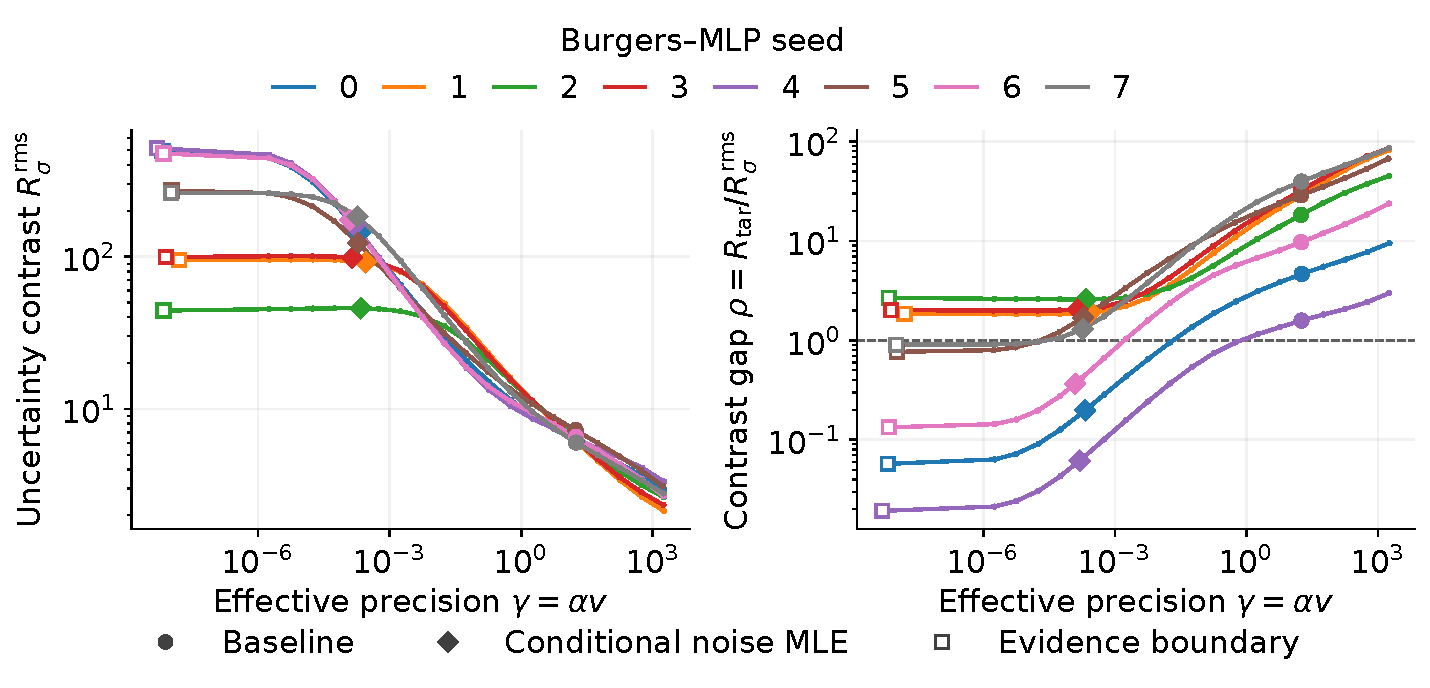
\includegraphics[width=0.96\textwidth]{figures/round2_contrast_and_gap.pdf}
\caption{Uncertainty contrast (left) and gap $\ratiogap=\Rtar/\Rrms$ (right) for eight
Burgers--MLP seeds with trained predictions fixed. Curves join $19$ unit-noise prior
settings and exact matched MLE/original-evidence points. Circles mark the baseline
$(\alpha_0,1)$, diamonds the conditional noise MLE $(\alpha_0,\widehat v)$, and open
squares the best original-grid evidence setting at the lower noise boundary. Selected
settings share contrasts with their unit-noise aliases, but not absolute widths. The
dashed line marks equal RMS contrasts, not calibration. Appendix~\ref{app:r2} summarises
other families, affine centres and extended-grid diagnostics; Appendix~\ref{oa:empirical} gives
their full curves.}
\label{fig:n1-scales}
\end{figure}

\emph{Training-based scale choices.}
The conditional MLE $\widehat v=\|r(\theta)\|^2/N$ fixes the trained parameter.
Fitted-residual reuse can underestimate variance; this plug-in residual scale is
not an unbiased discrepancy estimate. No classical degrees-of-freedom correction
is assigned here (Appendix~\ref{oa:numerics}). With trained centres it reverses
the allocation deficit in seeds $0$, $4$ and $6$; the other five have
$\ratiogap\in[1.30,2.59]$. Nevertheless, all eight seeds under-cover both regions:
one-standard-deviation coverage is $0.198$--$0.416$ in bulk and $0.018$--$0.5315$ in sharp;
at $1.96$ standard deviations it is $0.412$--$0.721$ and $0.051$--$0.698$.

On both zero-mean-prior evidence grids, $14/17$ best tested pairs lie at the lowest allowed noise
variance; extending the range does not resolve those boundary selections.
The three Allen--Cahn Fourier candidates are interior, whereas singular-value
perturbations substantially change Allen--Cahn MLP selections. These are finite-grid
candidates rather than reliably identified scales. Appendix~\ref{app:r2:evidence}
records the projected-data mechanism, extension and numerical sensitivity.

\emph{Predictive centres and linearisation.}
At the baseline, the zero-mean-prior affine centre increases full-grid error RMS in $14/17$ checkpoints
(Table~\ref{tab:r2-centres}). For Burgers--MLP, mean $\Rtar$ falls from $130.6$ to $13.13$
and mean $\ratiogap$ from $20.47$ to $2.09$, but mean sharp error RMS rises from $0.1138$
to $0.2448$ and bulk error RMS from $0.000805$ to $0.01821$; sharp error worsens in seven
of eight seeds. Thus a reduced target can accompany worse prediction.

The displacement separates as $\delta_\gamma=\delta_{L,\gamma}+\delta_{P,\gamma}$,
where the likelihood term is the shift under the $\theta$-centred prior and
$\delta_{P,\gamma}=-\gamma(F+\gamma I)^{-1}\theta$ is prior shrinkage. Its QR-complement
term is $-\theta_c$ at every scale, where $\theta_c$ is the parameter projection
onto that complement. At the baseline, total displacement is
$99.78$--$99.96\%$ of $\|\theta\|$, whereas the likelihood term is at most
$0.0155\%$. Prediction-level bounds establish prior-only worsening in all $14$
affected runs (Appendix~\ref{app:r3:centres}); parameter norms alone would not
establish that attribution.

For the $\theta$-centred prediction, the pointwise baseline shift bound ranges from
$0.00749$ to $0.0908$ standard deviations. Bounds establish $\rho>1$ in $16/17$;
direct evaluation gives $\rho>1$ in all $17$, resolving Burgers--MLP seed $4$ with gap $1.582$.
Both regions over-cover at one standard deviation. At the conditional-MLE
scales, $\rho^\theta\in[2.18,10.01]$. The affine mean improves full-grid RMS error
in $15/17$ runs (Table~\ref{tab:r2-centres}), with median error ratio $0.7953$.
At one standard deviation, all $17$ bulk regions over-cover and $12/17$ sharp regions
under-cover. Thus prediction can improve without
regional calibration. The residual variance is not re-estimated after shifting.

At the baseline, nonlinear evaluation $u_{\theta+\delta_{L,\gamma}}$ also retains
$\rho>1$ in all $17$, with regional RMS affine remainder below $6.4\times10^{-4}$
of RMS $\sigma$. At the MLE, however, the bulk remainder is $2.495$--$386.16$ times
RMS $\sigma$, despite $\|\delta_L\|/\|\theta\|\in[0.00782,0.03867]$.
Full-grid error worsens in $11/17$ and bulk error in all $17$.
Observed nonlinear gaps below one reflect bulk deterioration, not repaired allocation.
These are forward diagnostics with covariance frozen at $\theta$.

\emph{Oracle: contrast agreement and coverage.}
A descriptive oracle rescales each saved covariance to target $68\%$ bulk coverage using the
higher empirical quantile of $|e|/\sigma$, separately for each centre and time subset.
It uses reference errors and is not a practical tuning rule. For the five trained-centre
bracketing seeds, the closest saved points have $\ratiogap\in[0.954,1.032]$, yet sharp
coverage is $0.343$--$0.652$ at one standard deviation and $0.692$--$0.864$ at $1.96$.
For zero-mean-prior affine post-formation predictions, the closest points across all eight seeds have
$\ratiogap\in[0.933,1.193]$ and sharp one-standard-deviation coverage $0.009$--$0.347$.
At the five refined trained-centre roots, direct sharp coverage is
$0.30325$--$0.55725$ at one standard deviation and $0.67725$--$0.852$ at $1.96$
(Table~\ref{tab:r3-roots}). All values lie within the positive-modal envelopes,
whose upper bounds are at most $0.563$ and $0.862$, respectively
(Appendix~\ref{app:r3:root-envelope}). Contrast agreement therefore does not
restore sharp coverage under this bulk calibration.

At these five trained-centre roots, the $\theta$-centred affine prediction has
full-grid error RMS $0.493$--$0.973$ times that of the trained prediction and
$\rho^\theta\in[1.13,7.58]$; these precisions do not match its own error contrast.
After its own bulk-$68\%$ calibration, sharp one-standard-deviation coverage is
$0.1165$--$0.424$.

For $Z_j=e_j/\sigma_j$, define the variance-weighted regional second moment
\[
 M_r=\frac{\sum_{j\in r}\sigma_j^2Z_j^2}{\sum_{j\in r}\sigma_j^2}
     =\frac{\langle e^2\rangle_r}{\langle\sigma^2\rangle_r},\qquad
 \rho^2=M_{\mathcal S}/M_{\mathcal B}.
\]
Thus $\rho=1$ equates weighted second moments, leaving ordinary coverage quantiles
undetermined. At the five nearest saved oracle settings, using bulk-calibrated widths,
sharp median $|Z|$ ranges
over $[0.725,1.273]$, compared with $[0.655,0.701]$ in bulk; sharp $99$th percentiles
are $3.60$--$8.70$, versus $3.05$--$4.66$ in bulk. Sharp signed means include
$-1.96$ (seed $5$) and $0.85$ (seed $7$). The top $1\%$ of sharp points carry $15.3$--$23.8\%$ of error
energy, and width--absolute-error Spearman rank correlations are $0.693$--$0.936$.
Larger sharp medians show that the difference extends beyond extreme tails;
regional sign bias and substantial width--error ordering coexist with undercoverage.

An RMS deficit can coexist with overcoverage: seed $1$ has closest gap $1.836$
and sharp one-standard-deviation coverage $0.8605$; seed $3$ has gap $1.992$
and coverage $0.725$ (Tables~\ref{tab:r2-oracle} and~\ref{tab:r4-oracles}).

Sharp calibration using its higher empirical $0.68$ quantile gives sharp
$1.96$-standard-deviation coverage $0.8345$--$0.95775$ for Burgers--MLP, below
$0.95$ in $7/8$ runs. Other families and time subsets include overcoverage
(Table~\ref{tab:r4-oracles}): matching one quantile need not match another.
This output rescaling preserves within-region width patterns and does not test
a residual-informed likelihood that changes $J^\top D^{-1}J$.

In the sampled band $0.9\le\rho\le1.1$, Burgers--MLP seed $7$ has seven
settings with sharp one-standard-deviation coverage $0.44725$--$0.986$ after
bulk calibration: $\rho=0.925$ gives $0.756$, while $\rho=1.064$ gives $0.44725$.
These include undercoverage and overcoverage, without a continuous-band claim
(Appendix~\ref{app:r4-oracles}).

\emph{Ensemble comparison.}
An ensemble \citep{lakshminarayanan2017ensembles} of the eight Burgers--MLP runs, with
spread computed at divisor $K=8$, has $\Rrms=136.5$, its own mean-prediction target
$\Rtar=158.2$ and $\ratiogap=1.16$. Sharp $\meanZ=0.64$ and coverage is $0.876/0.993$
at $68/95\%$, while bulk $\meanZ=0.45$. It nearly matches allocation but does not restore
absolute calibration. The ordering against individual Gaussians depends on their scale:
at the conditional MLE three trained-centre gaps are below one and five lie in
$[1.30,2.59]$, each relative to its own predictor's error. Omitting one ensemble member
gives gaps $1.055$--$1.351$, sharp $68\%$ coverage $0.4935$--$0.9075$ and $95\%$ coverage
$0.9720$--$0.9995$. Omitting seed~$5$ gives the largest gap and lowest $68\%$ coverage;
its sharp error has correlation $-0.7517$ with the other seven's mean error. These ranges
measure membership sensitivity, not confidence intervals: each omission changes the
predictor, target and spread.


\subsection{Feature Expressivity for the Reference Solution}\label{sec:offmanifold}

The trained network's $129$ last-layer features, including the bias, can approximate
the sharp-region reference accurately when their readout is refitted using reference
values. This tests feature expressivity, separately from the coefficients selected by
residual-only training or the affine posterior. Let $\Phi$ be the feature matrix on the $80{,}000$ evaluation points
and $e=u_\theta-u^\ast$ the sampled trained-network error.

\begin{samepage}
\begin{definition}[Per-region fraction and masked-global ratio]\label{def:diagnostics}
For a region $r$ with nonzero error $e_r$ and local feature matrix $\Phi_r$, let $P_r$ denote the
orthogonal projector onto $\mathrm{col}(\Phi_r)$ and define the \emph{per-region} fraction
\begin{equation}\label{eq:fperregion}
  f^{\perp}_r \;=\; \frac{\|e_r - P_r e_r\|^2}{\|e_r\|^2}.
\end{equation}
Let $P$ instead denote the projector onto $\mathrm{col}(\Phi)$ formed once globally, and define
the \emph{masked-global} ratio
\begin{equation*}
  \tilde f^{\perp}_r \;=\; \frac{\big\|(e - Pe)\big|_r\big\|^2}{\|e_r\|^2}.
\end{equation*}
\end{definition}
\end{samepage}

The linear readout gives
$u_\theta|_r\in\mathrm{col}(\Phi_r)$. Since $e_r=u_\theta|_r-u^\ast|_r$,
\[
 (I-P_r)e_r=-(I-P_r)u^\ast|_r,
 \qquad
 f_r^\perp=\frac{\|(I-P_r)u^\ast|_r\|^2}{\|e_r\|^2}.
\]
The numerator is local reference-approximation error; the denominator is trained-network
error. Their regional ordering therefore depends on both.

\begin{samepage}
\begin{remark}[The per-region diagnostic is a fraction]\label{prop:wellposed}
For any self-adjoint idempotent map $P$ and nonzero $e$,
$\|e\|^2=\|Pe\|^2+\|e-Pe\|^2$, so $f_r^\perp\in[0,1]$.
\end{remark}

\begin{proof}
Self-adjointness and idempotence give $\langle e,Pe\rangle=\|Pe\|^2$;
expanding $\|e-Pe\|^2$ gives the identity and both bounds.
\end{proof}
\end{samepage}

\begin{samepage}
\begin{remark}[The masked-global quantity is not a fraction]\label{prop:illposed}
The masked-global ratio can exceed one, because global orthogonality need not survive
restriction to a region.
\end{remark}

\begin{proof}
For $\varphi=(1,1)^\top$, $e=(1,1/10)^\top$ and $r=\{2\}$, the rank-one projection
is $P_\varphi e=(11/20)\varphi$, giving $\tilde f_r^\perp=81/4=20.25$.
\end{proof}
\end{samepage}

For comparison, $\tilde f_{\mathcal B}^\perp=3.30$ on Burgers--MLP seed $2$ and $4.4$
on a synthetic control with error concentrated in a $5\%$ subset.

\begin{table}[t]
\centering


\small
\begin{tabular}{@{}lccccc@{}}
\toprule
& \multicolumn{3}{c}{Same grid: $f^{\perp}_r$} & \multicolumn{2}{c}{Held-out sharp region} \\
\cmidrule(lr){2-4}\cmidrule(lr){5-6}
configuration & $\mathcal{B}$ & $\mathcal{T}$ & $\mathcal{S}$ & random & $10$-slice blocks \\
\midrule
Burgers, MLP (seed 2)                        & $0.002$ & $0.001$ & $\mathbf{0.0001}$ & $0.000146$ & $0.000455$ \\
Burgers, Fourier $\mathrm{FS}=2$ (seed 2)    & $0.071$ & $0.057$ & $\mathbf{0.0015}$ & $0.00163$ & $0.00670$ \\
Allen--Cahn, MLP (seed 0)                    & $0.230$ & $0.030$ & $\mathbf{0.0009}$ & $0.00139$ & $0.0324$ \\
Allen--Cahn, Fourier $\mathrm{FS}=1$ (seed 0)& $0.051$ & $0.017$ & $\mathbf{0.0007}$ & $0.000841$ & $0.00987$ \\
\bottomrule
\end{tabular}
\caption{Reference expressivity of $129$ last-layer features, including the bias.
Residual energies are normalised by trained-network regional error. Same-grid columns
give \eqref{eq:fperregion}; held-out columns pool both test directions for random halves
and alternating ten-slice time blocks.}
\label{tab:offmanifold}
\end{table}

\emph{Measured off-span fractions.} Across all $17$ runs,
$f_{\mathcal S}^\perp$ is the smallest regional fraction. Its maximum
is $0.011616$ (Burgers--MLP seed $4$): at least $98.8\%$ of sampled sharp error lies
in the local last-layer span. The bulk-to-sharp fraction ratio ranges from $9.37$ to
$542.5$ (the displayed runs span $18$--$266$). Span containment makes this residual
an upper bound for the full-network projection residual on the same points.

\emph{Held-out fits.}
Within each region we fit alternating ten-slice time blocks and test the remaining blocks,
then swap, using unregularised least squares of numerical rank $129$. The pooled test
residual energy, divided by total regional error energy, is below $4\%$ in $16/17$
sharp-region fits (median $0.72\%$). The worst fraction, $14.2\%$, is on Burgers--MLP seed $4$,
whose sharp error RMS $0.00362$ is the smallest among Burgers--MLP seeds; its test
residual RMS is $0.00136$, versus error RMS $0.283$ on seed $2$.
Random halves remain close to same-grid fits (Table~\ref{tab:offmanifold}), but blocked
transition residual exceeds error energy in $10/17$ runs.
Because the trained prediction $u_\theta$ lies in the last-layer span and each fit has
full column rank, fitting $e$ or $u^\ast$ yields the same held-out residual energy.
The pooled held-out residuals thus measure reference approximation by the local
feature span, using additional reference information.
These are local last-layer tests within the evaluation grid; span containment transfers
only the same-grid bound, not held-out performance or a single global coefficient vector.

\emph{Expressivity and coefficient selection.}
Regional refits use reference values, whereas \eqref{eq:affine-mean} selects coefficients
from the residual likelihood and zero-mean parameter prior. The predictive-centre analysis
in Section~\ref{sec:ceiling} attributes its prediction worsening to prior shrinkage.
Together, these diagnostics distinguish feature expressivity from coefficient selection;
they do not identify the cause of the trained error or its uncertainty mismatch.

\subsection{Spectral Weighting of Regional Variance}\label{sec:theory}
\label{sec:theory:bounds}\label{sec:mechanism}\label{sec:mechanism:loading}

Covariance allocation is a weighted sum of tangent energies. Its modal quotient
connects the scale curves to the trained features; coarse spectral bounds describe
what remains identifiable after grouping those modes.

\emph{Modal weights and limits.}
Let $F=V\Lambda V^\top$, with eigenvalues $\lambda_i\ge0$, largest eigenvalue
$\lambda_{\max}$ and orthonormal eigenvectors $v_i$, and write
$c_i(x)=g(x)^\top v_i$. At unit noise,
\begin{equation}\label{eq:sigma-sum}
 \sigma^2(g)=g^\top(\alpha I+F)^{-1}g
           =\sum_i\frac{c_i^2}{\lambda_i+\alpha}.
\end{equation}
For residual variance $v$, each term is $v c_i^2/(\lambda_i+\gamma)$,
$\gamma=\alpha v$. Defining $a_{r,i}=\langle c_i(x)^2\rangle_r$ gives
\begin{equation*}\tag{3a}\label{eq:modal-quotient}
 (\Rrms(\gamma))^2=
 \frac{\sum_i a_{\mathcal S,i}/(\lambda_i+\gamma)}
      {\sum_i a_{\mathcal B,i}/(\lambda_i+\gamma)}.
\end{equation*}
For these finite sums,
\[
 \lim_{\gamma\to\infty}\Rrms=\sqrt{A_{\mathcal S}/A_{\mathcal B}},
 \quad A_r=\langle\|g\|^2\rangle_r,
 \qquad
 \lim_{\gamma\downarrow0}\Rrms=\sqrt{K_{\mathcal S}/K_{\mathcal B}},
 \quad K_r=\langle\|\Pi_{\ker J}g\|^2\rangle_r,
\]
provided $A_{\mathcal B}>0$ and $K_{\mathcal B}>0$, respectively. Multiplication
by $\gamma$ gives both termwise limits. The QR-complement ratio equals the
whole-kernel ratio when $J$ has full row rank. For $A_{\mathcal S},A_{\mathcal B}>0$,
at strong precision, writing
$\mu_r=\sum_i a_{r,i}\lambda_i/A_r$ gives the more precise expansion
\begin{equation}\label{eq:r3-strong-expansion}
 (\Rrms(\gamma))^2=\frac{A_{\mathcal S}}{A_{\mathcal B}}
 \left[1-\frac{\mu_{\mathcal S}-\mu_{\mathcal B}}{\gamma}
       +O\!\left(\frac{\lambda_{\max}^2}{\gamma^2}\right)\right].
\end{equation}
This follows by expanding each $(\lambda_i+\gamma)^{-1}$ and dividing the two
sums. Neither endpoint bounds intermediate contrast, and monotonicity need not
hold. For example,
$\lambda=(0,1,100)$, $a_{\mathcal B}=(1,1,100)$ and
$a_{\mathcal S}=(1,100,1)$ give both limits equal to $1$, but
$\Rrms(1)=\sqrt{10304/503}\approx4.53$.
The measured curves and strong-precision checks are in
Appendix~\ref{app:r2:modal}. The conditional limits and counterexample are
Lean-verified (Table~\ref{tab:lean}); expansion~\eqref{eq:r3-strong-expansion}
remains outside verification.
Figure~\ref{fig:n1-scales} changes the modal weights while holding the trained
tangents fixed. The predictive centres share the covariance contrast but have different error targets.

\emph{Two-subspace bounds.} We group the modes by a spectral cutoff.
\begin{samepage}
\begin{definition}[Spectral split and regional loadings]\label{def:split}
At threshold $\epsilon>0$, let $\Pi_{\rm sl}$ project onto modes with
$\lambda_i\le\epsilon$ and $\Pi_{\rm st}$ onto those with $\lambda_i>\epsilon$.
Define
\begin{equation*}
 Q_{r,\rm sl}=\langle\|\Pi_{\rm sl}g\|^2\rangle_r,
 \qquad Q_{r,\rm st}=\langle\|\Pi_{\rm st}g\|^2\rangle_r.
\end{equation*}
\end{definition}
\end{samepage}
For an individual vector, the lower and upper envelopes are
\begin{equation}\label{eq:variance-envelopes}
 \begin{aligned}
 m_\epsilon(g)&=\frac{\|\Pisl g\|^2}{\alpha+\epsilon}
              +\frac{\|\Pist g\|^2}{\alpha+\lambda_{\max}},\\
 M_\epsilon(g)&=\frac{\|\Pisl g\|^2}{\alpha}
              +\frac{\|\Pist g\|^2}{\alpha+\epsilon}.
 \end{aligned}
\end{equation}

Theorem~\ref{thm:ceiling}, proved in Appendix~\ref{app:aggregation}, bounds each
pointwise variance between these envelopes. Averaging its termwise inequalities
gives the primary regional bound
\begin{equation}\label{eq:regional-rms-sandwich}
 L_{\rm reg}(\epsilon)\le(\Rrms)^2\le U_{\rm reg}(\epsilon).
\end{equation}
Here $L_{\rm reg}(\epsilon)=\langle m_\epsilon(g)\rangle_{\mathcal S}/\langle M_\epsilon(g)\rangle_{\mathcal B}$
and $U_{\rm reg}(\epsilon)=\langle M_\epsilon(g)\rangle_{\mathcal S}/\langle m_\epsilon(g)\rangle_{\mathcal B}$,
assuming positive total bulk energy. This is exact
finite-sum aggregation, without a Jensen step. For common variance $v$, replace
$\alpha$ by $\gamma$; the common factor cancels. The envelopes are sharp over
spectra compatible with these summaries (Proposition~\ref{prop:sharp}, proved in
Appendix~\ref{app:sharpness}), but they discard energy placement within each block.
They can therefore remain wide even after intersecting thresholds.
Appendix~\ref{app:aggregation} treats secondary aggregations; Appendix~\ref{oa:lean},
Table~\ref{tab:lean}, records the formal verification scope.

\par\emph{Measured spectrum and loadings.}
With float64 machine epsilon $\varepsilon_{64}=2^{-52}$, the canonical Gram eigensolves
return positive eigenvalues spanning $19.6$--$21.2$ decades, but values below
$\varepsilon_{64}\lambda_{\max}$ are not individually resolved.
The inverse lifts $J^\top w_i/\sqrt{\lambda_i}$, where $w_i$ is a unit eigenvector
of $JJ^\top$, are unstable near that scale. We instead resolve the separated strong subspace and compute
\begin{equation*}
 \|\Pisl g\|^2=\|g\|^2-\|\Pist g\|^2.
\end{equation*}
This includes Fisher-null directions without division by small eigenvalues.
Orthonormality, cutoff separation, eigenpair error and independent variance checks
are described in Appendix~\ref{app:spectralchecks}.

% Generated by analysis/loading_table_tex.py; do not edit by hand.
\newcommand{\LoadingBMLPPerPoint}{259.5}
\newcommand{\LoadingBMLPMeanTangent}{514.9}
\newcommand{\LoadingBMLPCoherenceQuotient}{1.98}
\newcommand{\LoadingBMLPRMSBandAtAlpha}{[0.05,\,307.9]}
\newcommand{\LoadingBFourierPerPoint}{43.7}
\newcommand{\LoadingBFourierMeanTangent}{195.4}
\newcommand{\LoadingBFourierCoherenceQuotient}{4.48}
\newcommand{\LoadingBFourierRMSBandAtAlpha}{[0.06,\,103.5]}
\newcommand{\LoadingACMLPPerPoint}{59.3}
\newcommand{\LoadingACMLPMeanTangent}{268.6}
\newcommand{\LoadingACMLPCoherenceQuotient}{4.53}
\newcommand{\LoadingACMLPRMSBandAtAlpha}{[0.10,\,113.9]}
\newcommand{\LoadingACFourierPerPoint}{79.0}
\newcommand{\LoadingACFourierMeanTangent}{1132.4}
\newcommand{\LoadingACFourierCoherenceQuotient}{14.33}
\newcommand{\LoadingACFourierRMSBandAtAlpha}{[0.17,\,55.9]}
\newcommand{\LoadingSeedPerPointMin}{171.2}
\newcommand{\LoadingSeedPerPointMax}{268.0}
\newcommand{\LoadingSeedPerPointFactor}{1.56}
\newcommand{\LoadingSeedMeanTangentMin}{380.6}
\newcommand{\LoadingSeedMeanTangentMax}{742.0}
\newcommand{\LoadingSeedMeanTangentFactor}{1.95}
\newcommand{\LoadingCanonicalPerPointMin}{43.7}
\newcommand{\LoadingCanonicalPerPointMax}{259.5}

% Generated by analysis/recompute_saved_summaries.py; outward rounding of recorded inputs.
\newcommand{\RMSBoundBurgersMLPLower}{0.0488}
\newcommand{\RMSBoundBurgersMLPUpper}{307.86}
\newcommand{\RMSBoundBurgersFourierLower}{0.0648}
\newcommand{\RMSBoundBurgersFourierUpper}{103.51}
\newcommand{\RMSBoundAllenCahnMLPLower}{0.0982}
\newcommand{\RMSBoundAllenCahnMLPUpper}{113.87}
\newcommand{\RMSBoundAllenCahnFourierLower}{0.1743}
\newcommand{\RMSBoundAllenCahnFourierUpper}{55.92}

\begin{table}[t]
\centering\small\setlength{\tabcolsep}{4pt}


\begin{tabular}{@{}lrrrrl@{}}
\toprule
 & returned & below & $Q_{\mathcal S,\rm sl}/$ & $M_{\mathcal S,\rm sl}/$ & RMS bracket\\
configuration & decades & roundoff & $Q_{\mathcal B,\rm sl}$ & $M_{\mathcal B,\rm sl}$ & \\
\midrule
Burgers--MLP, seed $2$ & $21.2$ & $82\%$ & $\LoadingBMLPPerPoint$ & $\LoadingBMLPMeanTangent$ & $[\RMSBoundBurgersMLPLower,\RMSBoundBurgersMLPUpper]$\\
Burgers--Fourier, seed $2$ & $19.9$ & $13\%$ & $\LoadingBFourierPerPoint$ & $\LoadingBFourierMeanTangent$ & $[\RMSBoundBurgersFourierLower,\RMSBoundBurgersFourierUpper]$\\
Allen--Cahn--MLP, seed $0$ & $20.4$ & $66\%$ & $\LoadingACMLPPerPoint$ & $\LoadingACMLPMeanTangent$ & $[\RMSBoundAllenCahnMLPLower,\RMSBoundAllenCahnMLPUpper]$\\
Allen--Cahn--Fourier, seed $0$ & $19.6$ & $26\%$ & $\LoadingACFourierPerPoint$ & $\LoadingACFourierMeanTangent$ & $[\RMSBoundAllenCahnFourierLower,\RMSBoundAllenCahnFourierUpper]$\\
\bottomrule
\end{tabular}
\caption{Canonical spectrum and baseline sub-$\alpha$ loadings. Returned decades include
unresolved positive eigenvalues; the next column is the fraction below
$\varepsilon_{64}\lambda_{\max}$. Primary loading uses
$Q_{r,\rm sl}=\langle\|\Pisl g\|^2\rangle_r$; the supporting mean-tangent loading
uses $M_{r,\rm sl}=\|\Pisl\langle g\rangle_r\|^2$. The final column gives
\eqref{eq:regional-rms-sandwich} at $\epsilon=\alpha$, in contrast units, rounded
outward from recorded energies. Only Burgers--MLP has replicated baseline loadings.}
\label{tab:spectrum}\label{tab:loading}
\end{table}

Sharp-to-bulk tangent-energy ratios are close to one on Burgers: bulk/transition/sharp
means are $134/136/141$ for MLP and $114/119/120$ for Fourier. The canonical
strong-precision RMS limits are $1.02,1.03,1.46,1.09$, whereas baseline configuration-mean
contrasts are $3.92$--$7.30$; covariance weighting supplies the amplification.
At $\epsilon=\alpha$, the sharp field loads the weak subspace
$\LoadingCanonicalPerPointMin$--$\LoadingCanonicalPerPointMax$ times more strongly
than bulk (Table~\ref{tab:loading}). All $11$ evaluated baseline brackets contain their measured RMS
contrasts but are too wide to establish a deficit relative to the error target.
For eight Burgers--MLP seeds, primary loading ratios span
$\LoadingSeedPerPointMin$--$\LoadingSeedPerPointMax$; supporting mean-tangent ratios
span $\LoadingSeedMeanTangentMin$--$\LoadingSeedMeanTangentMax$.

The full-grid study extends this geometry to all $17$ runs. Among the full-time sampled
curves, $13/17$ have both increasing and decreasing segments, and $12/17$ leave the
interval formed by the tangent and QR-complement ratios. The saved fields reach
$\gamma/\lambda_{\max}=6.28\times10^{-5}$--$2.96\times10^{-4}$. Evaluation of
their regional modal sums at $10^3\lambda_{\max}$ confirms approach to the
tangent-norm limit, within $1.94\times10^{-4}$ relative across all full and
Burgers post-formation curves. Small positive singular values are retained without
exact-null classification. The measured curves, conditional limits and coarse
brackets answer distinct questions (Appendix~\ref{app:r2:modal}).
\par
% The exploratory anisotropic-prior intervention and its auxiliary mathematics
% are outside this manuscript's scope.

\section{Discussion and Conclusion}\label{sec:discussion}

Regional allocation and coverage are distinct properties of this post-hoc
Gaussian. Likelihood and scales determine covariance allocation; the predictive
centre also changes the error target and coverage. The tested training-only
choices do not consistently calibrate both regions.

\emph{Predictive centre and linearisation.}
The baseline mismatch survives removal of zero-mean prior shrinkage. At weaker
precision, affine prediction can improve without regional calibration, and a
modest relative parameter shift can produce a large nonlinear remainder.

Held-out refits demonstrate feature expressivity, separately from coefficient
selection. Spectral weights explain scale dependence, but the conditional limits
do not bound intermediate contrast, and coarse envelopes cannot certify the
baseline deficit. Evidence boundaries and perturbation sensitivity leave
weak-precision scale selection unresolved.

\emph{Residual-informed likelihoods.}
Residual-informed or block-wise variances $D$ replace $F$ by $J^\top D^{-1}J$,
after factoring out global noise variance, changing spectral directions and
within-region allocation. The common-scale oracle does not test this model. The
rejected Kuramoto--Sivashinsky example links small aggregate residuals to large
solution errors, without ruling out useful local residual information. Such
likelihood design remains untested.

\emph{Limitations.}
The study covers two $1{+}1$-dimensional nonlinear equations and two architectures with
a shared sub-network/fusion-head design. Only Burgers--MLP supplies eight fully
admitted seeds; the remaining families are small selected samples. Admission thresholds,
raw residual weights and reference-based regions are experimental conventions.
Root-coverage envelopes concern the five observed trained-centre crossings and
the stated bulk calibration, rather than optimal joint calibration.

The $\theta$-centred prior is conditional on fitted parameters. Nonlinear forward
checks retain covariance at the original checkpoint; they do not establish a nonlinear
posterior approximation. Spectral calculations do not certify weak-mode forward accuracy
or exact rank. The synthetic
stress test exceeds its whole-grid evidence tolerance, despite agreement at selected
settings (Appendix~\ref{app:r2}). Held-out expressivity is last-layer and within-grid;
it does not establish off-grid or full-network held-out approximation. Transfer to
higher dimensions, other architectures and training objectives is untested.

\emph{Implications.}
Assess accuracy, regional contrast and coverage for each predictive centre;
ensemble sensitivity likewise warrants assessment of the particular ensemble.
The trained-centre Gaussian is a covariance diagnostic.
An archived random half-grid split-conformal illustration \citep{lei2018conformal} on the reference run,
using absolute-error scores at target $0.95$, gives marginal coverage $0.950$ but
bulk, transition and sharp coverage $0.98$, $0.99$ and $0.31$. This descriptive
finite-grid example shows how marginal coverage can conceal regional imbalance.

\emph{Code and data availability.}
Code, trained parameters, saved results and the Lean development are available at
\url{https://github.com/soumya1729/pinn-uq-scale-sensitivity}.
The tagged reproduction release supplies the saved-data archive and its checksum.

\emph{Conclusion.}
Under the specified likelihood, sharp intervals under-cover at all five trained-centre
roots despite bulk calibration and regional RMS contrast agreement. Allocation
and coverage therefore require separate regional checks for each run and
predictive centre.


\begin{samepage}
\acks{%.
Computations were performed on the Padmanabha high-performance computing facility at
the Indian Institute of Science Education and Research Thiruvananthapuram.
\emph{Funding in direct support of this work:} None.
\emph{Additional revenues related to this work:} None.
The authors declare no competing financial interests.}
\end{samepage}

\appendix
\raggedbottom
\section{Experimental and Reporting Details}\label{app:training}\label{app:conventions}

The following details supplement the model and admission rule in Section~\ref{sec:setting}.
Training uses float64 throughout. Each architecture has $20$ spatial and $20$ temporal
sub-networks of widths $[\,\cdot\,,64,64,1]$ feeding a $[40,128,128,1]$ fusion head.
Activations are $\tanh$, biases are initialised to zero and weights are drawn from
$\mathcal N(0,2/d_{\rm in})$. Fourier models use $16$ random features per axis, with
bandwidth $2$ for Burgers and $1$ for Allen--Cahn. Adam has learning rate $10^{-3}$,
with $5000$ Burgers steps and $15{,}000$ Allen--Cahn steps, followed by $50$ and $200$
Levenberg--Marquardt steps. Each LM step uses at most $100$ CG iterations, initial
damping $10^{-4}$ and minimum $10^{-12}$; it accepts at $\rho_{\rm LM}>0.25$, divides
damping by $3$ at $\rho_{\rm LM}>0.75$ and multiplies it by $4$ on rejection, allowing
at most $5$ consecutive rejections. Residual row counts and weights are given in
Section~\ref{sec:setting}; complete implementation settings are preserved with the code.

Reported multi-run means average per-run quantities. Every $\pm$ denotes the population
standard deviation with divisor $n$; ranges give observed minima and maxima.
The three-run control varies paired pulse-width/diffusivity settings at seed $0$.
Mean gaps are means of ratios, not ratios of mean contrasts: on Burgers--MLP they are
$20.47$ and $20.49$, respectively. Reference-error oracles are evaluation devices,
not training-based tuning rules.

A common $2\%$ admission cutoff retains $13/17$ of the original cohort:
$8/8$ Burgers--MLP, $3/3$ Burgers--Fourier, Allen--Cahn MLP seed $3$ and
Allen--Cahn Fourier seed $1$. The original $3\%$ Allen--Cahn cutoff remains a
convention, not a PDE-derived tolerance. The unchanged masks and saved fields
permit the subset comparison below; its two Allen--Cahn results are single-run
descriptions. In this subset, the baseline zero-mean affine error increases in
$10/13$ runs; direct $\theta$-centred baseline predictions give $\rho^\theta>1$ in
all $13$, including the one case unresolved by the $12/13$ bound.
With trained centres, conditional-MLE sharp coverage is below nominal in all $13$ runs:
$[0.018,0.62425]$ at one sigma and $[0.051,0.768]$ at $1.96$ sigma. Bulk
coverage is below nominal in $10/13$ and $12/13$ runs at those thresholds,
respectively. All eight Burgers--MLP findings and the five refined trained-centre
crossings remain in this subset by construction.

\emph{Linear-control context.}
The contextual linear control solves $u_t+a u_x=\nu u_{xx}$ with $a=1$ and a
periodic Gaussian pulse. Three of four MLP attempts pass admission; the admitted
seed-$0$ runs vary paired pulse-width/diffusivity settings. At the baseline their
uncertainty contrasts are $[1.086,1.331]$, error contrasts $[0.7816,0.9986]$ and
gaps $[0.6521,0.899]$. They are not part of the nonlinear $17$-run scale study.

\emph{Grid and spectral checks.}\label{app:grid}\label{app:spectralchecks}
The top-$5\%$ region rule alone does not establish feature resolution. For the sharpest
slice, the discrete integral width in cells is
\[
 W_{\rm cells}=\frac{\sum_j|\partial_xu^\ast(x_j,t)|}{\max_j|\partial_xu^\ast(x_j,t)|}.
\]
This effective discrete width avoids the crossing-count floor of the half-maximum
statistic; exceeding one cell does not establish continuum resolution. On nested
spatial subsamples with recomputed masks, primary RMS and secondary mean-width
contrasts change by at most $1.1\%$ between $n_x=400$ and $200$. This sampling-density
check concerns baseline contrasts, not convergence of oracle coverage. The canonical Gram spectral projectors were checked for
orthonormality, separation at the cutoff and eigenpair backward error; independent
Woodbury evaluations checked variances. The all-17 direct-$J$ checks are summarised
in Appendix~\ref{app:r2:numerics}, with numerical protocols in Appendix~\ref{oa:numerics}.

\section{Spectral Bounds and Aggregation}\label{app:aggregation}

We give the proofs supporting the two-subspace summaries
in Section~\ref{sec:theory} and their aggregation to regional statistics.

\begin{theorem}[Two-sided spectral sandwich]\label{thm:ceiling}
For $F\succeq0$, $\alpha,\epsilon>0$ and $g_\bk\ne0$,
\begin{equation}\label{eq:sandwich}
 L(\epsilon):=\frac{m_\epsilon(g_\sh)}{M_\epsilon(g_\bk)}
 \le\frac{\sigma^2(g_\sh)}{\sigma^2(g_\bk)}
 \le\frac{M_\epsilon(g_\sh)}{m_\epsilon(g_\bk)}=:U(\epsilon).
\end{equation}
Consequently, the ratio lies between $\sup_{\epsilon>0}L(\epsilon)$ and
$\inf_{\epsilon>0}U(\epsilon)$.
\end{theorem}
\begin{proof}
In the weak block, $\alpha\le\alpha+\lambda_i\le\alpha+\epsilon$; in the strong
block, $\alpha+\epsilon<\alpha+\lambda_i\le\alpha+\lambda_{\max}$.
Applying reciprocal bounds to \eqref{eq:sigma-sum} gives
$m_\epsilon(g)\le\sigma^2(g)\le M_\epsilon(g)$.
Both bulk envelopes are positive, so division in opposite directions gives the result.
\end{proof}

The primary statistic averages variance before taking square roots. The secondary
mean-width ratio is $\achratio=\langle\sigma(g)\rangle_{\mathcal S}/
\langle\sigma(g)\rangle_{\mathcal B}$. Uniform pairwise bounds also transfer to it:
if $\ell\sigma(g_b)\le\sigma(g_s)\le u\sigma(g_b)$ for every sharp--bulk pair, averaging
over both finite regions and dividing by positive bulk mean width gives
$\ell\le\achratio\le u$. This differs from evaluating variance at a region-mean tangent.

For regions with positive mean width, define
$\kappa_r=\sigma(\langle g\rangle_r)/\langle\sigma(g)\rangle_r$.
The covariance norm triangle inequality gives $0\le\kappa_r\le1$, and cancellation
of the two mean widths gives, when $\kappa_{\mathcal B}>0$,
\begin{equation}\label{eq:ratio-identity}
 \frac{\sigma(\langle g\rangle_{\mathcal S})}{\sigma(\langle g\rangle_{\mathcal B})}
 =\frac{\kappa_{\mathcal S}}{\kappa_{\mathcal B}}\achratio.
\end{equation}
Equation~\eqref{eq:ratio-identity} shows why mean-tangent loadings cannot replace
the primary pointwise energies. The following sharpness result concerns the
information in those energies.

\emph{Sharpness of the spectral bounds.}\label{app:sharpness}
The following construction shows what can be inferred from the four block energies alone.
It does not assert that measured networks attain the bounding envelopes.

\begin{proposition}[Sharpness]\label{prop:sharp}
Fix $\alpha>0$, $0<\epsilon<\lambda_{\max}$ and four nonnegative block energies,
with positive total bulk energy. Spectra and vectors realising these energies can
approach either endpoint of \eqref{eq:sandwich}.
\end{proposition}
\begin{proof}
For $\epsilon<\epsilon'\le\lambda_{\max}$, use four orthogonal modes with eigenvalues
$0,\epsilon,\epsilon',\lambda_{\max}$. To approach $U$, place the sharp weak and
strong energies at $0,\epsilon'$, and the bulk energies at $\epsilon,\lambda_{\max}$.
Square-root coordinates realise the prescribed energies and give
\[
 \frac{q_{\sh,\rm sl}/\alpha+q_{\sh,\rm st}/(\alpha+\epsilon')}
      {q_{\bk,\rm sl}/(\alpha+\epsilon)+q_{\bk,\rm st}/(\alpha+\lambda_{\max})}
 \longrightarrow U(\epsilon)\quad(\epsilon'\downarrow\epsilon).
\]
For $L$, place sharp energies at $\epsilon,\lambda_{\max}$ and bulk energies at
$0,\epsilon'$. The ratio then tends to $L(\epsilon)$. The strict inequality
$\epsilon'>\epsilon$ keeps that mode in the strong block.
\end{proof}


\section{Full-Grid Scale and Centre Diagnostics}\label{app:r2}

These diagnostics use all $17$ admitted checkpoints: Burgers--MLP seeds $0$--$7$,
Burgers--Fourier seeds $0,2,6$, and Allen--Cahn MLP/Fourier seeds $0,1,3$.
Trained parameters, raw weighted residuals, reference fields, $400\times200$ grids and
global percentile masks remain fixed. Recentring does not change admission. Affine means
use the frozen output; $u_{\theta+\delta_L}$ is a separate nonlinear diagnostic with
covariance still at $\theta$. The three-run families are exploratory. Appendix~\ref{app:n1} retains per-seed
Burgers--MLP results; Appendix~\ref{oa:empirical} gives extended curves and tables.

\emph{Burgers--MLP per-seed results.}\label{app:n1}
Table~\ref{tab:n1-scales} lists the eight trained-centre runs. Its minima use the
original grid and matched aliases, whereas the all-17 diagnostics also include expanded
evidence and sensitivity-selected settings.

\begin{table}[ht]
\centering\small\setlength{\tabcolsep}{4pt}


\begin{tabular}{@{}rrrrrrrr@{}}
\toprule
 & & & & \multicolumn{2}{c}{bulk coverage} & \multicolumn{2}{c}{sharp coverage}\\
seed & baseline $\ratiogap$ & MLE $\ratiogap$ & min. sampled $\ratiogap$
 & $68\%$ & $95\%$ & $68\%$ & $95\%$\\
\midrule
0 & 4.66 & 0.20 & 0.06 & 0.261 & 0.501 & 0.516 & 0.684 \\
1 & 28.83 & 1.91 & 1.84 & 0.274 & 0.455 & 0.095 & 0.273 \\
2 & 18.33 & 2.59 & 2.59 & 0.380 & 0.598 & 0.137 & 0.349 \\
3 & 32.10 & 2.04 & 1.99 & 0.198 & 0.412 & 0.143 & 0.339 \\
4 & 1.58 & 0.06 & 0.02 & 0.233 & 0.449 & 0.531 & 0.630 \\
5 & 28.82 & 1.70 & 0.77 & 0.416 & 0.721 & 0.018 & 0.051 \\
6 & 9.74 & 0.37 & 0.13 & 0.247 & 0.459 & 0.363 & 0.698 \\
7 & 39.69 & 1.30 & 0.91 & 0.356 & 0.617 & 0.060 & 0.161 \\
\bottomrule
\end{tabular}
\caption{Original Burgers--MLP scale study at the fixed trained centre. Baseline and MLE gaps
use $(\alpha_0,1)$ and $(\alpha_0,\widehat v)$. Minima use the original $19$ unit-noise prior multipliers and
matched MLE/evidence points. Coverage is at the conditional MLE, within one and $1.96$
standard deviations.}
\label{tab:n1-scales}
\end{table}

Approximate sampled crossing brackets in $\alpha v$ are
\[
\begin{aligned}
\text{seed }0:&\quad[0.0182150,0.0576010],&
\text{seed }4:&\quad[0.569767,1.80176],\\
\text{seed }5:&\quad[1.73345,5.48164]\times10^{-5},&
\text{seed }6:&\quad[5.61912,17.7692]\times10^{-4},\\
\text{seed }7:&\quad[1.78416,5.64201]\times10^{-5}.&&
\end{aligned}
\]
These intervals need not contain unique roots.
No sampled crossing is found for seeds $1$--$3$; this does not exclude unsampled crossings.



\emph{Settings and computation.}\label{app:r2:numerics}
The unit-noise sweep uses $19$ prior multipliers $10^{-7}$--$10^2$, with exact aliases
for conditional-MLE and evidence-selected effective precisions. The evidence grids
span $\alpha/\alpha_0=10^{-7}$--$10^7$ and initially
$v/\widehat v=10^{-4}$--$10^6$ in quarter decades; one extension lowers the noise edge
to $10^{-8}\widehat v$. Six prescribed spectral sensitivity cases supply further
settings. For each prior centre, shared $\gamma=\alpha v$ gives the same contrast and affine mean;
widths differ by $\sqrt v$, without added predictive noise.

One direct-$J$ Householder QR/SVD per checkpoint gives
$J^\top=Q_1U\operatorname{diag}(s_i)V^\top$, with $Q=[Q_1,Q_c]$.
All $N=6400$ singular directions and $P-N$ complement coordinates are retained,
without a Gram matrix, rank cutoff or noise floor. Prediction/loss reconstruction and
baseline width comparisons give maximum width relative discrepancy
$5.41\times10^{-11}$. At all $401$ settings, independent differentiation checks
$h_\gamma=J^\top(r+J\delta_\gamma)+\gamma(\theta+\delta_\gamma)$.
The maximum normwise backward error is $6.19\times10^{-17}$ against a $10^{-7}$
tolerance; complement norm, projection, output and null-membership checks have maximum
scaled defect $5.10\times10^{-16}$. These consistency checks do not certify weak-mode
forward accuracy or exact rank. Appendix~\ref{oa:numerics} specifies their denominators.

The checkpoint-conditional $\theta$-centred comparison uses the same fixed-scale
covariance; Appendix~\ref{oa:numerics} records its separate $95$ checks.

\emph{Regional modal sums and conditional limits.}\label{app:r2:modal}
Let $\lambda_i=s_i^2$,
$q_{r,i}=\langle(U^\top Q_1^\top g(x))_i^2\rangle_r$,
$d_r=\langle\|Q_c^\top g(x)\|^2\rangle_r$, and
$A_r=d_r+\sum_iq_{r,i}$. Equation~\eqref{eq:modal-quotient} becomes
\begin{equation}\label{eq:r2-regional-modal}
 H_r(\gamma)=\frac{d_r}{\gamma}+\sum_i\frac{q_{r,i}}{\lambda_i+\gamma},\qquad
 \langle\sigma^2\rangle_r=vH_r(\gamma),\qquad
 \Rrms(\gamma)^2=\frac{H_{\mathcal S}(\gamma)}{H_{\mathcal B}(\gamma)}.
\end{equation}
The conditional limits in Section~\ref{sec:theory} follow by multiplying \eqref{eq:r2-regional-modal}
by $\gamma$: the strong limit requires $A_{\mathcal B}>0$, and the finite weak
ratio requires positive bulk energy in the whole kernel. The QR-complement ratio
in Table~\ref{tab:r2-limits} equals that weak limit if $J$ has full row rank;
tiny positive returned singular values do not certify this premise.

% Derived only from frozen production/review archives; no new grid or checkpoint evaluation.
\begin{table}[t]
\centering\small\setlength{\tabcolsep}{4pt}


\begin{tabular}{@{}lrrr@{}}
\toprule
family & strong-$\gamma$ ratio & QR-complement ratio & sampled $\Rrms$ \\
\midrule
Burgers--MLP & $[0.9467,\,1.023]$ & $[42.71,\,509.9]$ & $[2.136,\,517.3]$ \\
Burgers--Fourier & $[1,\,1.027]$ & $[11.81,\,30.54]$ & $[1.361,\,31.56]$ \\
Allen--Cahn--MLP & $[1.457,\,1.474]$ & $[1.268,\,2.532]$ & $[1.465,\,7.731]$ \\
Allen--Cahn--Fourier & $[1.089,\,1.138]$ & $[25.21,\,35.47]$ & $[2.822,\,31.08]$ \\
\bottomrule
\end{tabular}
\caption{Full-time regional RMS tangent-norm ratios, QR-complement ratios and measured contrast ranges across every saved $\gamma$ and admitted run in each family. The QR column equals the whole-kernel weak limit when $J$ has full row rank. Endpoint ratios are not global contrast bounds; the final column is a finite sampled range shared by all predictive centres.}
\label{tab:r2-limits}
\end{table}


Neither limit bounds the intermediate quotient in general. Of the $17$ full-time
sampled curves, $13$ have increasing and decreasing segments, and $12$ leave the
interval between the reported endpoint ratios. Allen--Cahn MLP has tangent/QR ratios
about $1.27$--$2.53$ but sampled maxima $7.30$--$7.73$. The largest saved
$\gamma/\lambda_{\max}$ is only $6.28\times10^{-5}$--$2.96\times10^{-4}$; the
saved modal sums also permit evaluation at stronger precisions without new fields.
At $\gamma=10^3\lambda_{\max}$, all full and Burgers post-formation contrasts are
within $1.94\times10^{-4}$ relative to their tangent-norm limits. The first-order
expansion \eqref{eq:r3-strong-expansion} differs from the returned squared ratios by
at most $3.43\times10^{-7}$ relative to those squared ratios.
Appendix~\ref{oa:empirical} reports changed-scale brackets and loading
ratios at $\epsilon=\gamma$; the brackets remain too broad to certify a realised-error deficit.

\emph{Evidence selection and mechanism.}\label{app:r2:evidence}
For the zero-mean prior's affine observation $y=J\theta-r$, set $z=V^\top y$ and
$C_i=v+\lambda_i/\alpha$. The affine log evidence \citep{mackay1992interpolation} is
\[
 \ell(\alpha,v)=-\tfrac12\sum_{i=1}^N[z_i^2/C_i+\log C_i+\log(2\pi)].
\]
Fourteen original selections occur at $10^{-4}\widehat v$ and remain on the new
$10^{-8}\widehat v$ boundary after extension; the three Allen--Cahn Fourier selections
are interior and unchanged (Table~\ref{tab:r2-evidence-summary}).
All selected alpha coordinates are interior. These zero-mean-prior selections are
best tested grid pairs, not continuous optima.

For the $\theta$-centred prior the same formula uses $z=-V^\top r$. On the extended
grid, $14$ selections lie at the lower noise boundary, two Allen--Cahn Fourier
selections at the upper alpha boundary, and one is interior. Sharp $1.96$-sigma
coverage around its affine mean is below nominal in all $17$ runs,
ranging from $0.00275$ to $0.90175$.

\begin{table}[t]
\centering\small\setlength{\tabcolsep}{4pt}


\begin{tabular}{@{}lrrr@{}}
\toprule
family & runs & extended noise edge & selected $\gamma/\gamma_{\rm ext}$ \\
\midrule
Burgers--MLP & $8$ & $8/8$ & $[0.562,3.162]$ \\
Burgers--Fourier & $3$ & $3/3$ & $[1,1.778]$ \\
Allen--Cahn--MLP & $3$ & $3/3$ & $[1.778,3.16228\times10^5]$ \\
Allen--Cahn--Fourier & $3$ & $0/3$ & $1$ \\
\bottomrule
\end{tabular}
\caption{Zero-mean-prior evidence-grid outcomes and six-case sensitivity. The interval is perturbed
selected effective precision divided by the extended selection, across each family's
runs and cases. Perturbations change singular values and the affine observation
coherently, keeping singular vectors fixed; fields at alternative selected scales use
the original Jacobian. Appendix~\ref{oa:empirical} gives full per-run values.}
\label{tab:r2-evidence-summary}
\end{table}

Each case changes singular values by
$\delta s=\varepsilon_{64}\max(N,P)s_{\max}$ or $10\delta s$, upwards, downwards or
alternately, with zero clamping. It also changes
$z$ coherently by $(s'-s)\theta_{\rm modes}$, where
$\theta_{\rm modes}=U^\top Q_1^\top\theta$. These are finite sensitivity cases, not
certified error bounds. All Allen--Cahn MLP selections change in all six cases;
their $1\times$ quadratic terms $\delta s^2/\gamma$ alone are $7.55$, $488.55$ and
$228.65$. Their extended selections are not treated as robust scale estimates.

At fixed alpha,
\begin{equation}\label{eq:r2-evidence-slope}
 D_v=\frac{\partial\ell}{\partial\log v}
 =-\frac12\sum_i\frac{v}{C_i}\left(1-\frac{z_i^2}{C_i}\right).
\end{equation}
At the fourteen extended boundary selections, the $\lambda_i/\gamma<0.01$ group
contains $603$--$4594$ modes, with summed projected data energy only
$0.000481$--$0.014164$ times summed model variance
(Figure~\ref{fig:r2-evidence-energy} illustrates Burgers--MLP seed~$2$).
Its negative slope contributions
favour lower noise. Original/extended fixed-alpha slopes are $-2633$ to $-2561$ /
$-2379$ to $-2255$ for Burgers--MLP, $-481$ to $-417$ / $-407$ to $-317$ for
Burgers--Fourier, and $-1503$ to $-1124$ / $-1397$ to $-753$ for Allen--Cahn MLP.
Allen--Cahn Fourier slopes are $-291$ to $-113$; an interior quarter-decade maximum
need not have zero continuous slope. These fixed-alpha slopes describe local behaviour,
not an alpha-reoptimised path or the limit $v\to0$.

\begin{figure}[t]
\centering
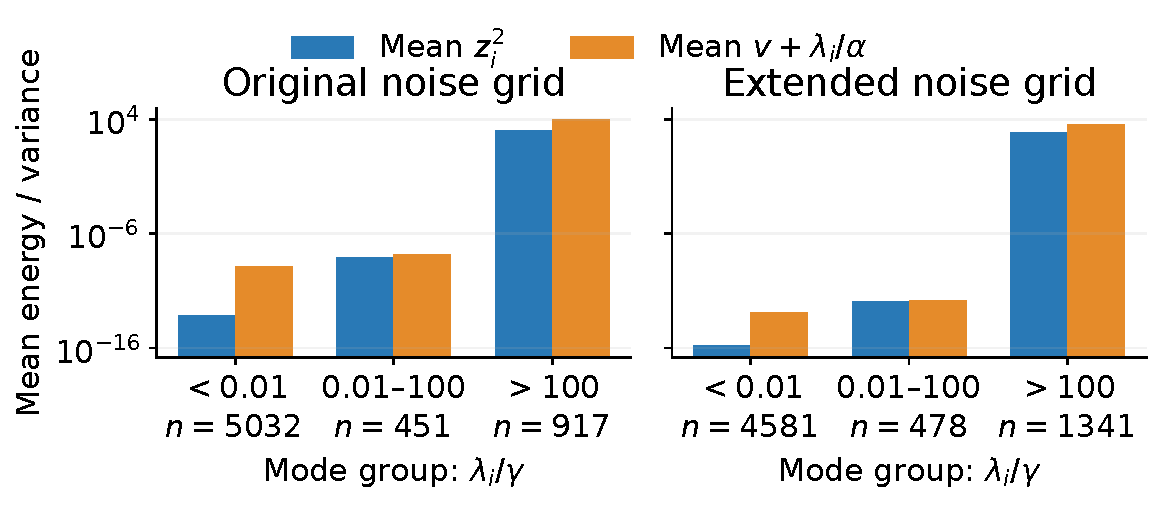
\includegraphics[width=.86\textwidth]{figures/round2_evidence_energy_reference.pdf}
\caption{Burgers--MLP seed $2$, zero-mean prior: projected affine-observation energy $z_i^2$ and model
variance $v+\lambda_i/\alpha$ at the original and extended selections, averaged in three
$\lambda_i/\gamma$ groups. Counts accompany the bars. Little data energy in weak
groups favours lower noise in \eqref{eq:r2-evidence-slope}; the grouping is descriptive.}
\label{fig:r2-evidence-energy}
\end{figure}

\emph{Synthetic validation.}
Dense tests give posterior mean/covariance relative discrepancies at most
$4.90\times10^{-12}$ and $3.01\times10^{-12}$, and log-evidence discrepancy
$1.42\times10^{-13}$. Across $1000$ correctly specified draws, posterior-centred
coverage is $0.6870$ (SE $0.00544$) at one sigma and $0.9534$ (SE $0.00249$) at
$1.96$ sigma. A full-column-rank fit with $N=40,P=12,v=0.2$ gives mean residual-noise
MLE $0.140411$ (SE $0.001198$), consistent with $(N-P)v/N=0.14$ rather than $v$.
In each $100$-draw evidence toy, including a $21.2$-decade spectrum with $79/96$
eigenvalues below $\varepsilon_{64}\lambda_{\max}$, all selected pairs are interior and
agree with the prescribed-spectrum reference. The stressed toy nevertheless fails its
whole-grid $10^{-7}$ scaled tolerance, with maximum discrepancy
$4.55\times10^{-5}$, despite selected log-evidence discrepancies at most
$9.40\times10^{-8}$. Appendix~\ref{oa:numerics} gives scale-estimation distributions and
the failed check; these controls do not establish PINN evidence stability.

\emph{Centre and regional displacement.}\label{app:r2:centres}
Table~\ref{tab:r2-centres} compares the prior centres and nonlinear diagnostic at fixed
baseline/MLE scales; Table~\ref{tab:r2-relative-shift} reports relative regional
displacements. A reduced error contrast need not improve accuracy. Covariance
is shared, whereas errors and coverage are centre-specific.
At the conditional MLE, all eight Burgers--MLP zero-mean-prior affine gaps lie in
$[1.51,3.39]$; one-standard-deviation coverage is $0.9815$--$0.99998$ in bulk
and $0.4185$--$0.92475$ in sharp. The trained-centre allocation reversals and
bulk undercoverage therefore do not transfer to this centre.

% Generated by scripts/make_paper_tables.py from reviewed theta outputs.
\begin{table}[t]
\centering\small\setlength{\tabcolsep}{3pt}
\begin{tabular}{@{}lrr*{6}{r}@{}}
\toprule
 & & & \multicolumn{3}{c}{Baseline} & \multicolumn{3}{c}{Conditional MLE} \\
\cmidrule(lr){4-6}\cmidrule(l){7-9}
family & $n$ & trained & zero & $\theta$ & nonlinear & zero & $\theta$ & nonlinear \\
\midrule
Burgers--MLP & $8$ & $0.02546$ & $0.05883^{(7)}$ & $0.02537^{(2)}$ & $0.02537^{(2)}$ & $0.023^{(5)}$ & $0.02283^{(2)}$ & $0.03944^{(6)}$ \\
Burgers--Fourier & $3$ & $0.05124$ & $0.04316^{(1)}$ & $0.05118^{(0)}$ & $0.05118^{(0)}$ & $0.04235^{(0)}$ & $0.04935^{(0)}$ & $0.05091^{(1)}$ \\
Allen--Cahn--MLP & $3$ & $0.03287$ & $0.2776^{(3)}$ & $0.03275^{(0)}$ & $0.03275^{(0)}$ & $0.02804^{(1)}$ & $0.02455^{(0)}$ & $0.2701^{(3)}$ \\
Allen--Cahn--Fourier & $3$ & $0.03351$ & $0.245^{(3)}$ & $0.03349^{(0)}$ & $0.03349^{(0)}$ & $0.03975^{(1)}$ & $0.02496^{(0)}$ & $0.03861^{(1)}$ \\
\bottomrule
\end{tabular}
\caption{Paired full-grid RMS prediction errors. Entries are unweighted means
of per-run RMS errors; superscripts count runs worse than the trained predictor
out of $n$. Baseline uses $(\alpha_0,1)$ and MLE uses $(\alpha_0,\widehat v)$.
Zero and $\theta$ denote the two affine prior-centre predictions; nonlinear
is $u_{\theta+\delta_L}$, a forward diagnostic rather than a posterior mean.
All comparisons retain the original covariance linearisation.}
\label{tab:r2-centres}
\end{table}


\begin{table}[t]
\centering\small\setlength{\tabcolsep}{4pt}


\begin{tabular}{@{}llrr@{}}
\toprule
family & region & baseline & MLE \\
\midrule
Burgers--MLP & bulk & $[7.54,54.1]$ & $[0.264,1.51]$ \\
 & sharp & $[0.58,57.7]$ & $[0.108,8.55]$ \\
Burgers--Fourier & bulk & $[3.87,8.31]$ & $[0.823,2.42]$ \\
 & sharp & $[0.666,0.864]$ & $[0.167,0.809]$ \\
Allen--Cahn--MLP & bulk & $[15.7,23]$ & $[1.57,2.59]$ \\
 & sharp & $[5.46,7.22]$ & $[0.416,0.628]$ \\
Allen--Cahn--Fourier & bulk & $[8.94,9.95]$ & $[0.97,1.09]$ \\
 & sharp & $[4.38,6.25]$ & $[0.36,2.26]$ \\
\bottomrule
\end{tabular}
\caption{Across-run ranges of total regional RMS zero-mean-prior affine displacement divided by trained
error RMS on the same full-time region. Baseline is $(\alpha_0,1)$ and MLE is
$(\alpha_0,\widehat v)$. Displacement alone does not determine prediction accuracy;
its alignment with trained error matters. Appendix~\ref{oa:empirical} includes transition
regions and evidence settings.}
\label{tab:r2-relative-shift}
\end{table}

\emph{Sampled oracle and post-formation coverage.}
At every saved $\gamma$, centre and subset, a higher empirical bulk-$0.68$ quantile of
$|e_c|/\sigma$ supplies a width multiplier. Selection minimises $|\log\rho|$ across
distinct saved precisions, with lowest $\gamma$ breaking ties. This reference-error
oracle uses sampled settings. Trained Burgers--MLP
seeds $0,4,5,6,7$ have full-time sampled crossing brackets; six zero-mean affine full-time
and six post-formation curves have brackets. Full-time zero-mean affine seeds $1,7$ and
post-formation seeds $1,3$ stay above one at every saved point.

% Derived only from frozen production/review archives; no new grid or checkpoint evaluation.
\begin{table}[t]
\centering\footnotesize\setlength{\tabcolsep}{4pt}


\begin{tabular}{@{}llrrrr@{}}
\toprule
family & subset & trained $68\%$ & affine $68\%$ & trained $95\%$ & affine $95\%$ \\
\midrule
Burgers--MLP & full & $[0.3427,\,0.8605]$ & $[0.164,\,0.9815]$ & $[0.639,\,0.9742]$ & $[0.298,\,0.995]$ \\
Burgers--MLP & post & $[0.1639,\,0.9959]$ & $[0.008972,\,0.3467]$ & $[0.4176,\,1]$ & $[0.01387,\,0.7121]$ \\
Burgers--Fourier & full & $[0.1985,\,0.5978]$ & $[0.2828,\,0.4662]$ & $[0.4472,\,0.7588]$ & $[0.5145,\,0.742]$ \\
Burgers--Fourier & post & $[0.01713,\,0.0938]$ & $[0.08972,\,0.3173]$ & $[0.03589,\,0.1819]$ & $[0.1998,\,0.5571]$ \\
Allen--Cahn--MLP & full & $[0.0095,\,0.0655]$ & $[0.2015,\,0.2755]$ & $[0.0395,\,0.2722]$ & $[0.3588,\,0.3962]$ \\
Allen--Cahn--Fourier & full & $[0.1477,\,0.2005]$ & $[0.0775,\,0.3827]$ & $[0.2407,\,0.4138]$ & $[0.1432,\,0.7338]$ \\
\bottomrule
\end{tabular}
\caption{Across-run sharp-region coverage ranges for trained and zero-mean-prior affine centres at each run's closest saved contrast setting, chosen separately for each centre and subset. A closest sample need not have $\rho\approx1$, so these rows do not generally evaluate coverage after RMS-contrast matching. At each saved $\gamma$, a higher empirical bulk-$0.68$ quantile supplies the width multiplier; selection minimises $|\log\rho|$ and the lowest saved $\gamma$ breaks exact ties. These reference-error oracles use all $8$ Burgers--MLP or $3$ other admitted runs, including runs without a crossing. ``Post'' uses the unchanged global masks intersected with Burgers $t\ge1/\pi$. Bulk one-sigma coverage is about $0.68002$; neither nominal sharp coverage nor an exact root is enforced.}
\label{tab:r2-oracle}
\end{table}


For Burgers, post-formation masks intersect unchanged global masks with
$t\ge1/\pi$, yielding $48{,}246$ bulk, $4928$ transition and $1226$ sharp points.
Table~\ref{tab:r2-oracle} includes all runs, including those without crossings; the
closest sample need not have $\rho\approx1$. Its coverage ranges distinguish regional
contrast from calibration. Saved modal sums refine the five trained-centre crossings;
direct root fields confirm their coverage envelopes (Table~\ref{tab:r3-roots}).
These precisions are not contrast-matching roots for the other centres.
Appendix~\ref{oa:empirical} gives per-run curves.

\emph{Predictive bounds for the prior-centre comparison.}\label{app:r3:centres}
For $\gamma,v>0$, write $A_\gamma=F+\gamma I$. The zero-mean-prior shift splits as
\[
 \delta_\gamma=\delta_{L,\gamma}+\delta_{P,\gamma},\qquad
 \delta_{L,\gamma}=-A_\gamma^{-1}J^\top r,\qquad
 \delta_{P,\gamma}=-\gamma A_\gamma^{-1}\theta.
\]
In the factorisation above, their coordinates are
$-s_i(V^\top r)_i/(s_i^2+\gamma)$ and
$-\gamma\theta_{\rm modes,i}/(s_i^2+\gamma)$; the QR-complement contributions
are $0$ and $-Q_cQ_c^\top\theta$, respectively. The total norm includes their
cross term. Replacing the prior by $\vartheta\sim\mathcal N(\theta,\alpha^{-1}I)$
removes $\delta_{P,\gamma}$ and leaves the covariance unchanged.

Define $\mathcal K_\gamma=r^\top J A_\gamma^{-1}J^\top r$ and
$c_\gamma=\sqrt{\mathcal K_\gamma/v}$. Since
$\delta_{L,\gamma}^\top A_\gamma\delta_{L,\gamma}=\mathcal K_\gamma$,
Cauchy--Schwarz in the $A_\gamma$ metric gives the pointwise bound
\begin{equation}\label{eq:r3:centre-bound}
 |m^\theta_\gamma(x)-u_\theta(x)|
 =|g(x)^\top\delta_{L,\gamma}|
 \le\sigma(x)c_\gamma,\qquad
 \mathcal K_\gamma=\sum_i\frac{s_i^2(V^\top r)_i^2}{s_i^2+\gamma}.
\end{equation}
Let $E_r$ and $\Sigma_r$ denote trained error RMS and uncertainty RMS, and let
$q_{r,i}$ be the regional mode energies in \eqref{eq:r2-regional-modal}.
The regional RMS triangle inequality also gives
\begin{equation}\label{eq:r3:regional-bound}
 B_r=\min\!\left\{c_\gamma\Sigma_r,
              \sum_i|\delta_{L,\gamma,i}|\sqrt{q_{r,i}}\right\},\qquad
 \max(0,E_r-B_r)\le E^\theta_r\le E_r+B_r.
\end{equation}
For $E^\theta_{\mathcal B}>0$ and $\Rrms>0$,
$\rho^\theta\ge\max(0,E_{\mathcal S}-B_{\mathcal S})/
[(E_{\mathcal B}+B_{\mathcal B})\Rrms]$.
The prior-only prediction differs from
the archived zero-mean affine mean by $g^\top\delta_L$; its full-grid error is
therefore at least $E^{\rm zero}_{\rm full}-B_{\rm full}$. This attributes
worsening through a prediction-level bound rather than parameter norms.
If $C_c(t)$ denotes empirical coverage at $t$ standard deviations, then
\[
 C_{\rm trained}(t-c_\gamma)\le C_\theta(t)
       \le C_{\rm trained}(t+c_\gamma),\qquad t\ge c_\gamma,
\]
by the pointwise triangle inequality.

\input{round3_math_results}

\emph{Coverage envelopes at refined contrast-matching roots.}\label{app:r3:root-envelope}
At unit noise, each pointwise variance has the positive modal representation
$q_\gamma(x)=\sum_i a_i(x)/(\lambda_i+\gamma)$, including the QR complement
as a zero-eigenvalue mode, with $a_i(x),\lambda_i\ge0$.
For positive endpoint variances at saved precisions
$0<l\le\gamma\le h$, $l<h$, and
$t=(\gamma-l)/(h-l)$, positivity gives
\begin{equation}\label{eq:r3:variance-envelope}
 L_\gamma=\frac{(1-t)lq_l+thq_h}{\gamma}
 \le q_\gamma\le
 U_\gamma=\left(\frac{1-t}{q_l}+\frac{t}{q_h}\right)^{-1}.
\end{equation}
For the lower bound in \eqref{eq:r3:variance-envelope}, $\gamma q_\gamma$ is concave because every
$\gamma/(\lambda_i+\gamma)$ is concave. For the upper bound,
$q'=-\sum_i a_i/(\lambda_i+\gamma)^2$ and
$q''=2\sum_i a_i/(\lambda_i+\gamma)^3$ satisfy
$(q')^2\le qq''/2$ by Cauchy--Schwarz. Hence
$(1/q)''=[2(q')^2-qq'']/q^3\le0$, and taking the reciprocal of its chord gives
$U_\gamma$. Both envelopes decrease with $\gamma$ since $q_l\ge q_h$.

For a numerically refined root bracket $[a,b]\subset[l,h]$, use $L_b$ and
$U_a$ to retain root-location uncertainty. The higher empirical bulk-$0.68$
quantile $Q_{\mathcal B}$ is monotone, so
\[
 k_{\min}=Q_{\mathcal B}(|e|/\sqrt{U_a}),\qquad
 k_{\max}=Q_{\mathcal B}(|e|/\sqrt{L_b})
\]
enclose the multiplier $k_\gamma$ that calibrates bulk coverage at the root.
For sharp coverage at threshold $z\ge0$, this yields
\begin{equation}\label{eq:r3:coverage-envelope}
 \left\langle\mathbf1\{|e|\le z k_{\min}\sqrt{L_b}\}\right\rangle_{\mathcal S}
 \le C_{\mathcal S,\gamma}(z)\le
 \left\langle\mathbf1\{|e|\le z k_{\max}\sqrt{U_a}\}\right\rangle_{\mathcal S}.
\end{equation}
These analytic bounds use the returned spectral model and saved endpoint fields;
they are not directed-rounding certificates for the original Jacobian.
Direct pointwise root evaluations confirm the enclosures in Table~\ref{tab:r3-roots}.
Root refinement concerns the five observed
trained-centre brackets, without asserting uniqueness or global optimality.
Appendix~\ref{oa:lean} maps the Lean verification of these analytic bounds.
The evaluated run counts and refined brackets remain numerical results.

\input{round3_math_root_table}


\emph{Regional calibration and sampled agreement band.}\label{app:r4-oracles}
At each trained-centre closest saved setting, use either
$k_{\mathcal B}=Q_{\mathcal B}(|e|/\sigma;0.68)$ or
$k_{\mathcal S}=Q_{\mathcal S}(|e|/\sigma;0.68)$, with the higher empirical quantile.
Write $C^r_{\mathcal S}(z)=\langle\mathbf1\{|e|\le z k_r\sigma\}\rangle_{\mathcal S}$
and $Z^r=e/(k_r\sigma)$ for the resulting coverage and standardised errors.
Table~\ref{tab:r4-oracles} gives full-grid per-seed results and family ranges,
including the Burgers post-formation subsets. Sharp calibration fixes its
one-standard-deviation coverage by construction: $0.68025$ on $4000$ full-grid
sharp points and $0.68108$ on $1226$ post-formation points here. The informative
outputs are coverage at $1.96$ standard deviations and the absolute and signed
standardised means. These are finite-grid descriptions, not repeated-draw guarantees.
Inclusive quantile comparisons can differ by one point from older multiplied-width
arithmetic; all continuous summaries reproduce to relative tolerance $10^{-12}$.

The band inventory retains every distinct saved precision with $0.9\le\rho\le1.1$:
$28$ run/subset settings across the full grids and Burgers post-formation masks.
For Burgers--MLP seed $7$, the seven full-grid samples give sharp coverage
$0.44725$--$0.986$ at one standard deviation and $0.78375$--$1$ at $1.96$ after
bulk calibration. Their $\rho$ values span $0.90635$--$1.06370$; nearby contrast
values need not correspond to nearby precisions on a nonmonotone curve.
The other four crossing seeds each have one saved full-grid point in the band,
with one-standard-deviation coverages $0.34275$, $0.437$, $0.35925$ and $0.5165$
for seeds $0,4,5,6$. The archived per-run inventory is sampled rather than a
continuous-band enclosure; Table~\ref{tab:r3-roots} retains the separate refined-root bounds.

% Recomputed from frozen round-two fields by analysis/round4_local/review_round4.py.
\begin{table}[!tb]
\centering\small\setlength{\tabcolsep}{4pt}
\begin{tabular}{@{}lrrrrrr@{}}
\toprule
Burgers--MLP seed & $\rho$ & $C^{\mathcal B}_{\mathcal S}(1)$ & $C^{\mathcal B}_{\mathcal S}(1.96)$ & $C^{\mathcal S}_{\mathcal S}(1.96)$ & $\overline{|Z|}^{\mathcal S}$ & $\overline Z^{\mathcal S}$\\
\midrule
0 & 0.95438 & 0.34275 & 0.7885 & 0.92025 & 0.91339 & $-0.24502$ \\
1 & 1.8363 & 0.8605 & 0.97425 & 0.865 & 0.94283 & $0.85765$ \\
2 & 2.5874 & 0.44675 & 0.639 & 0.85025 & 1.3644 & $1.209$ \\
3 & 1.9924 & 0.725 & 0.933 & 0.9175 & 0.77179 & $0.56348$ \\
4 & 0.95486 & 0.437 & 0.86375 & 0.95775 & 0.83109 & $-0.069397$ \\
5 & 0.97331 & 0.35925 & 0.69175 & 0.8345 & 1.0436 & $-1.0371$ \\
6 & 1.0323 & 0.5165 & 0.8435 & 0.92825 & 0.85021 & $0.069544$ \\
7 & 0.96422 & 0.65175 & 0.837 & 0.84675 & 1.034 & $0.79421$ \\
\midrule
\multicolumn{2}{l}{Family / subset ($n$)} & \multicolumn{2}{c}{$C^{\mathcal S}_{\mathcal S}(1.96)$} & $\overline{|Z|}^{\mathcal S}$ & \multicolumn{2}{c}{$\overline Z^{\mathcal S}$}\\
\midrule
\multicolumn{2}{l}{Burgers--MLP / full ($8$)} & \multicolumn{2}{c}{$[0.8345,\,0.95775]$} & $[0.77179,\,1.3644]$ & \multicolumn{2}{c}{$[-1.0371,\,1.209]$} \\
\multicolumn{2}{l}{Burgers--Fourier / full ($3$)} & \multicolumn{2}{c}{$[0.82475,\,0.85075]$} & $[1.0792,\,1.3448]$ & \multicolumn{2}{c}{$[0.98518,\,1.3234]$} \\
\multicolumn{2}{l}{Allen--Cahn--MLP / full ($3$)} & \multicolumn{2}{c}{$[0.921,\,0.959]$} & $[0.77708,\,0.86039]$ & \multicolumn{2}{c}{$[-0.29925,\,0.32371]$} \\
\multicolumn{2}{l}{Allen--Cahn--Fourier / full ($3$)} & \multicolumn{2}{c}{$[0.98325,\,0.9995]$} & $[0.71247,\,0.81491]$ & \multicolumn{2}{c}{$[-0.36263,\,0.27285]$} \\
\multicolumn{2}{l}{Burgers--MLP / post ($8$)} & \multicolumn{2}{c}{$[0.94454,\,1]$} & $[0.61868,\,0.98575]$ & \multicolumn{2}{c}{$[-0.87154,\,0.82267]$} \\
\multicolumn{2}{l}{Burgers--Fourier / post ($3$)} & \multicolumn{2}{c}{$[0.8646,\,1]$} & $[0.82852,\,0.87527]$ & \multicolumn{2}{c}{$[0.7548,\,0.86578]$} \\
\bottomrule
\end{tabular}
\caption{Trained-centre regional calibration at each run's closest saved contrast setting.
The superscript $\mathcal B$ or $\mathcal S$ denotes the region whose higher empirical
$0.68$ quantile supplies the width multiplier. The upper panel gives eight full-grid
Burgers--MLP seeds; the lower panel gives observed ranges for all $17$ full-grid runs
and the Burgers post-formation subsets. Each setting minimises $|\log\rho|$, with ties
at the lowest saved precision. $\overline{|Z|}^{\mathcal S}$ and $\overline Z^{\mathcal S}$
are absolute and signed means of sharp-calibrated standardised errors.
Sharp one-standard-deviation coverage is fixed by construction, up to discreteness
and ties. Displayed values are rounded; reference calibration does not define a training rule.}
\label{tab:r4-oracles}
\end{table}


\emph{Width versus allocation.}
At $v=1$, changing $\gamma$ changes modal weights. At fixed $\gamma=\alpha_0$,
varying $v$ with $\alpha=\alpha_0/v$ multiplies widths by $\sqrt v$ without changing
contrast: $\meanZ$ scales as $v^{-1/2}$ and coverage is the empirical CDF of fixed
standardised errors at $\sqrt v$. Figure~\ref{fig:r2-coverage-scale} shows both effects;
the fixed-$\gamma$ curves are rescalings of saved fields, not fitted scales.

\begin{figure}[!t]
\centering
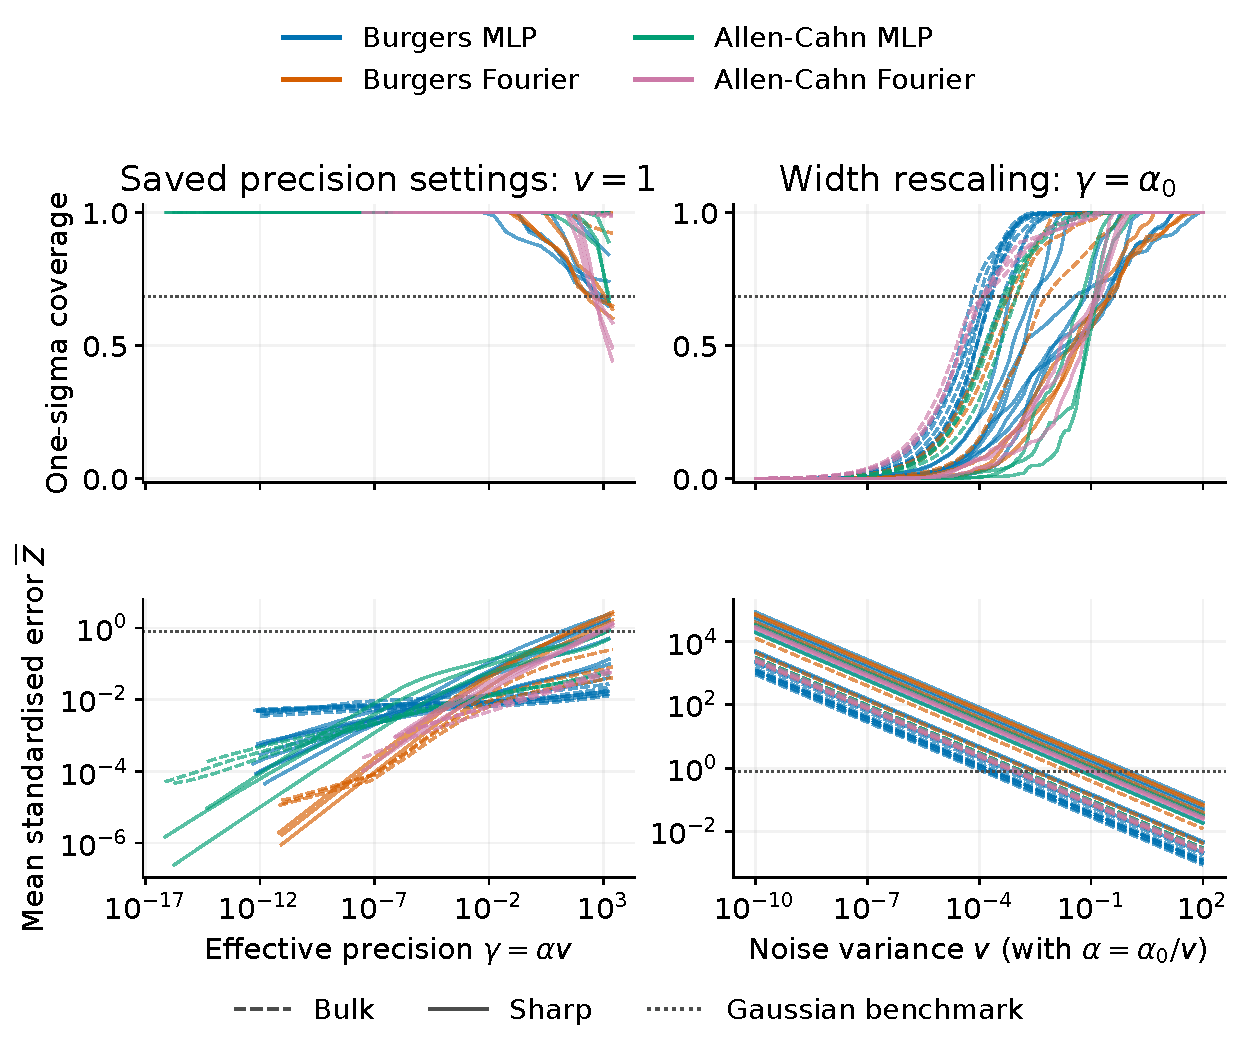
\includegraphics[width=.95\textwidth]{figures/round2_coverage_scale.pdf}
\caption{Trained-centre one-sigma coverage and mean standardised error for all $17$
full-time runs. Colours identify families; dashed/solid curves denote bulk/sharp.
Left: saved precisions at $v=1$; right: width rescaling at $\gamma=\alpha_0$.
Dotted lines mark Gaussian expectations $0.68269$ and $0.79788$.
Lines join evaluated points without asserting confidence intervals.}
\label{fig:r2-coverage-scale}
\end{figure}





\section{Extended Empirical Records}\label{oa:empirical}
The extended records use the fixed $17$-checkpoint cohort, global reference
masks and raw weighted residuals (Definitions~\ref{def:regions} and
\ref{def:gate}). Covariance contrast is shared by the predictive centres at fixed scales;
error contrast and the gap are centre-specific (Definition~\ref{def:metrics}).
``Full'' denotes the complete evaluation grid. Burgers ``post'' intersects the unchanged
masks with $t\ge1/\pi$; no Allen--Cahn post-formation subset is imposed.
Figures~\ref{fig:r2-full-burgers} and~\ref{fig:r2-full-ac} show covariance contrasts and
trained/zero-mean affine gaps; Table~\ref{tab:r2-centres} adds the $\theta$-centred comparison.

\subsection{Evidence Selections and Regional Spectral Summaries}
Table~\ref{tab:r2-evidence} extends the zero-mean-prior evidence summary in Appendix~\ref{app:r2}.
The initial evidence grid has lower noise edge $10^{-4}\widehat v$ and its one
extension has lower edge $10^{-8}\widehat v$. The six perturbation cases are specified in Appendix~\ref{oa:numerics}; selections
are finite-grid candidates and displayed ranges are descriptive.
% Derived only from frozen production/review archives; no new grid or checkpoint evaluation.


\emph{Changed-scale spectral partition.}
Let $q_{r,i}=\langle(U^\top Q_1^\top g)_i^2\rangle_r$ and
$d_r=\langle\|Q_c^\top g\|^2\rangle_r$, using the factorisation in Appendix~\ref{app:r2:numerics}.
At $\epsilon=\gamma$, these saved energies give
$Q_{r,\mathrm{sl}}=d_r+\sum_{\lambda_i\le\gamma}q_{r,i}$ and
$Q_{r,\mathrm{st}}=\sum_{\lambda_i>\gamma}q_{r,i}$.
Substitution into Equation~\eqref{eq:variance-envelopes}, with prior precision
replaced by $\gamma$, gives the returned-spectrum brackets in
Table~\ref{tab:r2-changed-bounds}. Table~\ref{tab:r2-scale-loadings} gives unweighted
energy ratios. Neither certifies weak-mode forward accuracy.
% Derived only from frozen production/review archives; no new grid or checkpoint evaluation.

% Derived from existing saved archives only.


\subsection{Displacement under the Zero-Mean Prior}
Table~\ref{tab:oa-relative-shift} extends Table~\ref{tab:r2-relative-shift} to transition
regions and evidence settings.
For the shift $c+b_\gamma$, the scale-independent component
$c(x)=-g(x)^\top Q_cQ_c^\top\theta$ gives $\langle(c+b_\gamma)^2\rangle_r=\langle c^2\rangle_r+
\langle b_\gamma^2\rangle_r+2\langle cb_\gamma\rangle_r$.
Every full-grid sharp complement field contains both signs. For Burgers--MLP, its
RMS is $0.001999$--$0.06048$ and signed mean $-0.02154$--$0.004895$; $4/8$ baseline
sharp cross terms are destructive. For Burgers--Fourier seed $0$, complement sharp
RMS $0.04236$ exceeds total MLE shift RMS $0.04102$. Component RMS values are nonadditive.
% Derived from existing saved archives only.

\begin{table}[!tbp]
\centering\footnotesize\setlength{\tabcolsep}{4pt}


\begin{tabular}{@{}lrrrrrr@{}}
\toprule
run & $a_{\rm orig}$ & $a_{\rm ext}$ & $v_{\rm ext}/\widehat v$ & $\gamma_{\rm ext}$ & perturbed $\gamma/\gamma_{\rm ext}$ & $\delta s^2/\gamma_{\rm ext}$ \\
\midrule
BM0 & $0.316$ & $0.316$ & $1\!\times\!10^{-8}$ & $6.64\!\times\!10^{-13}$ & $[1,\,3.16]$ & $0.0619$ \\
BM1 & $0.562$ & $0.562$ & $1\!\times\!10^{-8}$ & $1.59\!\times\!10^{-12}$ & $[1,\,1.78]$ & $0.0338$ \\
BM2 & $0.316$ & $0.562$ & $1\!\times\!10^{-8}$ & $1.24\!\times\!10^{-12}$ & $[0.562,\,1.78]$ & $0.0289$ \\
BM3 & $0.562$ & $0.562$ & $1\!\times\!10^{-8}$ & $7.87\!\times\!10^{-13}$ & $[1,\,1.78]$ & $0.0408$ \\
BM4 & $0.316$ & $0.316$ & $1\!\times\!10^{-8}$ & $4.95\!\times\!10^{-13}$ & $[1,\,3.16]$ & $0.0832$ \\
BM5 & $0.562$ & $0.562$ & $1\!\times\!10^{-8}$ & $1.06\!\times\!10^{-12}$ & $[1,\,1.78]$ & $0.0256$ \\
BM6 & $0.562$ & $0.562$ & $1\!\times\!10^{-8}$ & $6.99\!\times\!10^{-13}$ & $[1,\,1.78]$ & $0.0555$ \\
BM7 & $0.562$ & $0.562$ & $1\!\times\!10^{-8}$ & $1.03\!\times\!10^{-12}$ & $[1,\,1.78]$ & $0.0297$ \\
BF0 & $1$ & $1$ & $1\!\times\!10^{-8}$ & $6.71\!\times\!10^{-12}$ & $[1,\,1]$ & $0.00666$ \\
BF2 & $1$ & $1$ & $1\!\times\!10^{-8}$ & $8.52\!\times\!10^{-12}$ & $[1,\,1.78]$ & $0.00844$ \\
BF6 & $1$ & $1$ & $1\!\times\!10^{-8}$ & $9.23\!\times\!10^{-12}$ & $[1,\,1]$ & $0.00665$ \\
AM0 & $0.01$ & $5.62\!\times\!10^{-4}$ & $1\!\times\!10^{-8}$ & $4.88\!\times\!10^{-15}$ & $[1.78,\,1000]$ & $7.55$ \\
AM1 & $0.00316$ & $1.78\!\times\!10^{-5}$ & $1\!\times\!10^{-8}$ & $7.07\!\times\!10^{-17}$ & $[17.8,\,3.16\!\times\!10^{5}]$ & $489$ \\
AM3 & $0.00562$ & $3.16\!\times\!10^{-5}$ & $1\!\times\!10^{-8}$ & $1.69\!\times\!10^{-16}$ & $[5.62,\,3.16\!\times\!10^{5}]$ & $229$ \\
AF0 & $0.562$ & $0.562$ & $0.01$ & $8.03\!\times\!10^{-7}$ & $[1,\,1]$ & $4.83\!\times\!10^{-8}$ \\
AF1 & $0.316$ & $0.316$ & $0.00178$ & $3.11\!\times\!10^{-8}$ & $[1,\,1]$ & $1.63\!\times\!10^{-6}$ \\
AF3 & $0.562$ & $0.562$ & $0.0562$ & $4.85\!\times\!10^{-6}$ & $[1,\,1]$ & $6.6\!\times\!10^{-9}$ \\
\bottomrule
\end{tabular}
\caption{Zero-mean-prior evidence selections and six-case sensitivity. BM/BF and AM/AF denote
Burgers and Allen--Cahn MLP/Fourier, with seed suffixes; $a=\alpha/\alpha_0$.
BM/BF/AM select the lower noise edges specified above; AF selections are interior
and unchanged. The $1\times$ envelope $\delta s$ gives the quadratic term,
not a uniform eigenvalue error bound.}
\label{tab:r2-evidence}

\par\medskip
\centering\small\setlength{\tabcolsep}{4pt}


\begin{tabular}{@{}lrr@{}}
\toprule
family & conditional MLE & extended evidence \\
\midrule
Burgers--MLP & $[0.00491,\,7.01\!\times\!10^{4}]$ & $[0.00237,\,1.88\!\times\!10^{5}]$ \\
Burgers--Fourier & $[0.0258,\,1.13\!\times\!10^{3}]$ & $[0.0222,\,1.43\!\times\!10^{3}]$ \\
Allen--Cahn--MLP & $[0.0079,\,713]$ & $[0.00105,\,3.06\!\times\!10^{3}]$ \\
Allen--Cahn--Fourier & $[0.0161,\,1.15\!\times\!10^{3}]$ & $[0.0124,\,1.97\!\times\!10^{3}]$ \\
\bottomrule
\end{tabular}
\caption{Changed-scale two-block brackets at $\epsilon=\gamma$ from saved direct-$J$
regional energies, in $\sigma$-ratio units. Intervals enclose the union of run-specific returned-spectrum brackets, rounded outward. Weak-mode forward accuracy remains
uncertified, and the broad brackets cannot establish the realised-error deficit.}
\label{tab:r2-changed-bounds}
\end{table}
\begin{table}[p]
\centering\footnotesize\setlength{\tabcolsep}{4pt}


\begin{tabular}{@{}llrr@{}}
\toprule
family & setting & $Q_{\mathcal S,\mathrm{sl}}/Q_{\mathcal B,\mathrm{sl}}$ & $Q_{\mathcal S,\mathrm{st}}/Q_{\mathcal B,\mathrm{st}}$ \\
\midrule
Burgers--MLP & MLE & $[2.15\times10^{3},\,1.94\times10^{5}]$ & $[0.896,\,1.05]$ \\
 & original evidence & $[1.95\times10^{3},\,2.67\times10^{5}]$ & $[0.896,\,1.05]$ \\
 & extended evidence & $[1.91\times10^{3},\,2.67\times10^{5}]$ & $[0.896,\,1.05]$ \\
Burgers--Fourier & MLE & $[150,\,832]$ & $[0.999,\,1.05]$ \\
 & original evidence & $[150,\,998]$ & $[0.999,\,1.05]$ \\
 & extended evidence & $[145,\,996]$ & $[0.999,\,1.05]$ \\
Allen--Cahn--MLP & MLE & $[14,\,20.5]$ & $[2.12,\,2.17]$ \\
 & original evidence & $[4.59,\,9.76]$ & $[2.12,\,2.17]$ \\
 & extended evidence & $[2.14,\,7.02]$ & $[2.12,\,2.17]$ \\
Allen--Cahn--Fourier & MLE & $[291,\,693]$ & $[1.19,\,1.29]$ \\
 & original evidence & $[476,\,988]$ & $[1.19,\,1.29]$ \\
 & extended evidence & $[476,\,988]$ & $[1.19,\,1.29]$ \\
\bottomrule
\end{tabular}
\caption{Changed-scale sharp-to-bulk mean-square tangent loading ratios on the full-time regions. Entries give across-run ranges. At each saved setting, weak loading sums returned modes with $\lambda_i\le\gamma$ and the QR complement; stiff loading sums the remaining modes. Thus the partition uses $\epsilon=\gamma$, as in Table~\ref{tab:r2-changed-bounds}. These are energy ratios, without a square root or covariance weights, and are not uncertainty contrasts. The returned weak-mode split does not certify exact rank or weak-mode forward accuracy. Evidence settings are best tested zero-mean-prior grid selections.}
\label{tab:r2-scale-loadings}

\par\medskip
\centering\footnotesize\setlength{\tabcolsep}{4pt}


\begin{tabular}{@{}llrrrr@{}}
\toprule
family & region & baseline & MLE & original evidence & extended evidence \\
\midrule
Burgers--MLP & bulk & $[7.54,\,54.1]$ & $[0.264,\,1.51]$ & $[0.338,\,1.53]$ & $[0.349,\,1.49]$ \\
 & transition & $[9.07,\,109]$ & $[0.288,\,1.69]$ & $[0.266,\,1.53]$ & $[0.286,\,1.42]$ \\
 & sharp & $[0.58,\,57.7]$ & $[0.108,\,8.55]$ & $[0.114,\,14.9]$ & $[0.122,\,16.9]$ \\
Burgers--Fourier & bulk & $[3.87,\,8.31]$ & $[0.823,\,2.42]$ & $[0.714,\,1.97]$ & $[0.679,\,1.84]$ \\
 & transition & $[3.51,\,7.08]$ & $[0.955,\,1.8]$ & $[0.807,\,1.53]$ & $[0.804,\,1.42]$ \\
 & sharp & $[0.666,\,0.864]$ & $[0.167,\,0.809]$ & $[0.156,\,0.695]$ & $[0.155,\,0.762]$ \\
Allen--Cahn--MLP & bulk & $[15.7,\,23]$ & $[1.57,\,2.59]$ & $[2.43,\,10.9]$ & $[21.8,\,30.5]$ \\
 & transition & $[10.8,\,13.9]$ & $[0.868,\,1.64]$ & $[1.18,\,3.32]$ & $[4.05,\,21.2]$ \\
 & sharp & $[5.46,\,7.22]$ & $[0.416,\,0.628]$ & $[0.626,\,0.81]$ & $[0.626,\,5.07]$ \\
Allen--Cahn--Fourier & bulk & $[8.94,\,9.95]$ & $[0.97,\,1.09]$ & $[0.748,\,0.963]$ & $[0.748,\,0.963]$ \\
 & transition & $[9.86,\,11]$ & $[0.794,\,1.74]$ & $[0.631,\,1.13]$ & $[0.631,\,1.13]$ \\
 & sharp & $[4.38,\,6.25]$ & $[0.36,\,2.26]$ & $[0.331,\,1.45]$ & $[0.331,\,1.45]$ \\
\bottomrule
\end{tabular}
\caption{Regional RMS zero-mean-prior affine posterior-mean shift divided by trained-prediction RMS error, with both quantities evaluated on the same full-time region. Entries give across-run ranges ($8$ Burgers--MLP runs and $3$ in each other family). Baseline is $(\alpha_0,1)$; MLE is $(\alpha_0,\widehat v)$. Original and extended evidence columns use best tested grid settings, not certified continuous optima. A ratio above one means that the displacement exceeds the trained error in regional RMS; it does not determine whether the displaced prediction is more accurate.}
\label{tab:oa-relative-shift}
\end{table}

\FloatBarrier
\begin{figure}[p]
\centering
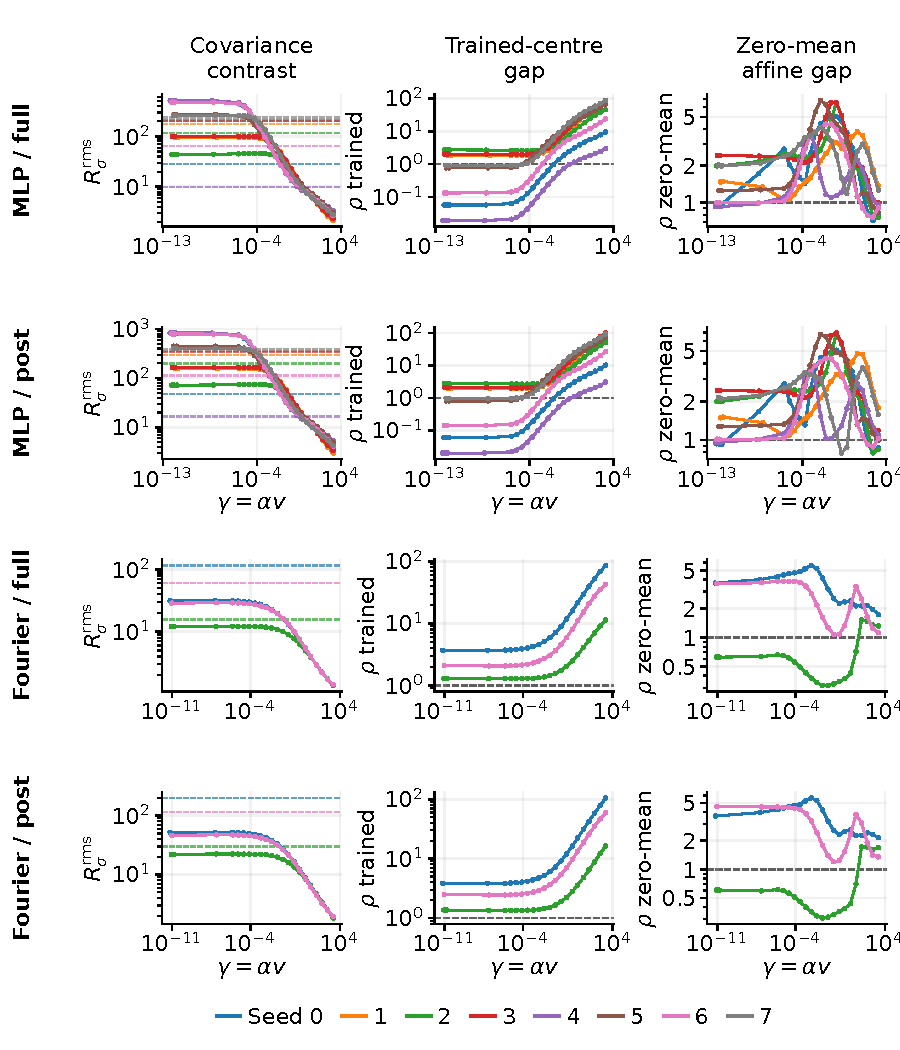
\includegraphics[width=.95\textwidth]{figures/round2_burgers_families_merged.pdf}
\caption{Burgers: eight admitted MLP and three admitted Fourier runs. Rows show MLP
full-grid/post-formation, then Fourier full-grid/post-formation; post-formation
intersects unchanged global masks with $t\ge1/\pi$. Columns show RMS covariance
contrast, trained gap and zero-mean affine gap; each gap uses its centre's error target.
Coloured dashed lines give trained error targets; grey lines mark $\rho=1$.
Every distinct saved $\gamma$, including extensions and sensitivity aliases, uses the
original Jacobian. Lines join samples without establishing monotonicity or a weak limit.}
\label{fig:r2-full-burgers}\label{fig:r2-full-bf}
\label{fig:r2-post-bm}\label{fig:r2-post}
\end{figure}

\clearpage
\begin{figure}[!tbp]
\centering
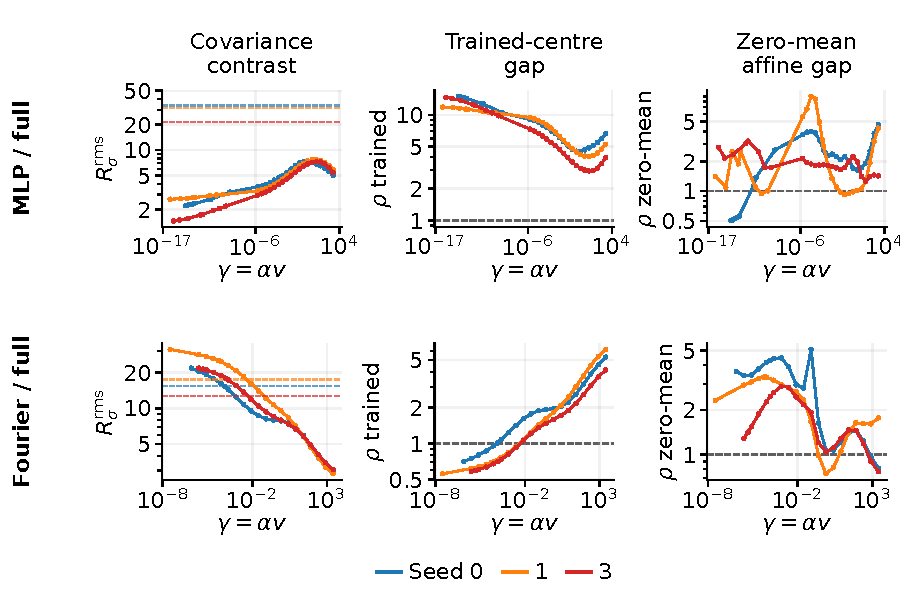
\includegraphics[width=.98\textwidth]{figures/round2_allen_cahn_families_merged.pdf}
\caption{Allen--Cahn full-grid scale and centre curves for three admitted MLP (top)
and three admitted Fourier (bottom) checkpoints. Columns and dashed lines follow
Figure~\ref{fig:r2-full-burgers}; each gap uses its centre's error target. Evidence
settings for both families are in Table~\ref{tab:r2-evidence}. All panels use the
original Jacobian; lines connect saved settings.}
\label{fig:r2-full-ac}\label{fig:r2-full-af}
\end{figure}

\section{Computation and Numerical Validation}\label{oa:numerics}
This record specifies the checks supporting Appendix~\ref{app:r2}; their
reported defects and interpretation remain separate from forward-accuracy certification.

\subsection{Direct-J Evaluation and Consistency Checks}
The factorisation, grids and zero-mean-prior results are in
Appendix~\ref{app:r2:numerics}. At all $401$ settings, automatic differentiation
independently checks
\begin{align*}
 h_\gamma&=J^\top(r+J\delta_\gamma)+\gamma(\theta+\delta_\gamma),\\
 \eta_{\rm back}&=\frac{\|h_\gamma\|}
 { (\lambda_{\max}+\gamma)\|\delta_\gamma\|
       +\|J^\top r+\gamma\theta\|}.
\end{align*}
Absolute residuals, denominators and shift norms are archived. Complement checks
use $J\delta_c$, norm, projection and output for
$\delta_c=-Q_cQ_c^\top\theta$. Normwise residuals can miss weak-direction errors;
null membership alone establishes neither amplitude nor completeness.

The $95$ distinct $\theta$-centred checkpoint--precision pairs merge repetitions
among baseline, conditional MLE, original/extended evidence under both priors,
and five trained-centre roots. Replacing $h_\gamma$ by
$J^\top(r+J\delta_L)+\gamma\delta_L$ and its denominator by
$(\lambda_{\max}+\gamma)\|\delta_L\|+\|J^\top r\|$ gives maximum ratio
$9.12\times10^{-17}$. Nonlinear evaluation retains $J$, $g$ and covariance at
$\theta$; independent NumPy predictions at nine points per setting agree within
$4.72\times10^{-12}$ absolute.

Fields reproduce regional metrics and spectral sums reproduce mean variances.
All $34$ zero-mean-prior evidence selections and one-log-unit sets
($\ell\ge\max_{\rm grid}\ell-1$) reproduce from
saved surfaces; all $34$ $\theta$-centred selections reproduce from corresponding factors.
Saved arrays reproduce the $401$ displacement norms and regional variances
(Appendix~\ref{app:r3:centres}). Envelopes contain every tested intermediate
variance field and a prescribed-spectrum null-mode example at $49$ interior
precisions; direct coverage at the five refined roots also lies within its
envelopes. These consistency
checks do not certify the original Jacobian by interval arithmetic.

\subsection{Evidence Sensitivity Protocol}
The six cases in Appendix~\ref{app:r2:evidence} retain singular vectors and change
the observation coherently by $z'=z+(s'-s)\theta_{\rm modes}$, where
$z=V^\top(J\theta-r)$ and $\theta_{\rm modes}=U^\top Q_1^\top\theta$.
An assumed singular-value budget gives
\[
 |\Delta\lambda_i|\le2s_i|\Delta s_i|+|\Delta s_i|^2.
\]
At $s_i=\sqrt\gamma$, the relative envelope is
$2\delta s/\sqrt\gamma+\delta s^2/\gamma$, with terms multiplied by $10$ and
$100$ in the $10\times$ case. The exposed Allen--Cahn MLP quadratic terms are
reported in Table~\ref{tab:r2-evidence}. Formed-Gram roundoff
(Table~\ref{tab:spectrum}) is not a direct-$J$ error bound.

All Allen--Cahn Fourier selections and Burgers--Fourier seeds $0,6$ are unchanged;
seed $2$ moves noise and $\gamma$ up one quarter decade in the increase-$10\times$
case. Every Burgers--MLP selection changes in at least two cases, retaining its
noise boundary, with alpha ratios $0.562$--$3.162$. Allen--Cahn MLP changes in all
six cases: noise ratios reach $177.8$ (seed $0$) and $3162$ (seeds $1,3$), and
$\gamma$ ratios reach $1000$ and $316{,}228$, respectively. Fixed-pair log-evidence
changes reach about $-1.05\times10^6$. The Allen--Cahn MLP scales are not
robust estimates; fields at alternative selections use the original Jacobian.

The derivative in \eqref{eq:r2-evidence-slope} groups modes by
$\lambda_i/\gamma<0.01$, $0.01$--$100$ and $>100$. For an isolated weak cluster,
its leading log-evidence contribution is
$-\tfrac12[m\log v+\sum_i z_i^2/v]$ plus a constant, suggesting
$v_*\approx m^{-1}\sum_i z_i^2$ at fixed $\alpha$ if all modes remain weak.
For exact-null modes with positive projected energy this expression is exact.
Positive modes can leave the cluster as $v$ falls; other modes affect the full
optimum. The grouped energies therefore explain a local boundary tendency,
without a goodness-of-fit test, an alpha-reoptimised path or a $v\to0$ conclusion.
Allen--Cahn Fourier has positive transition-group contributions partly offsetting
its negative weak group. Calculations retain the full formula; individual
coordinates within unresolved clusters are not interpreted.

Against a local central log-noise finite difference, the largest slope defect is
$4.43\times10^{-6}$ absolute or $5.51\times10^{-9}$ after scaling by $1+|D_v|$.
This verifies the calculation rather than evidence-model adequacy.

% Summary of unchanged synthetic archives; no new simulation or tolerance change.
\subsection{Synthetic Controls}\label{app:evidence-toys}
The small $12\times20$ design compares QR/SVD posterior means, covariances and evidence
with dense calculations, with maximum discrepancies $4.90\times10^{-12}$ and
$3.01\times10^{-12}$ in relative norm and $1.42\times10^{-13}$ in absolute log evidence.
In $1000$ correctly specified prior/noise draws, the affine posterior output mean gives
one-sigma coverage $0.6870$ (draw-level SE $0.00544$) and $95\%$ coverage $0.9534$
(SE $0.00249$). A separate full-column-rank least-squares example with $N=40,P=12$
and generating noise variance $v=0.2$ gives a mean of $0.140411$ (SE $0.001198$)
for the fitted-residual estimator $\|r_{\rm fit}\|^2/N$, consistent with
$(N-P)v/N=0.14$. In a general linear fit the factor is
$(N-\operatorname{rank}(X))/N$, reducing to $(N-P)/N$ only for full column rank.
For a full-row-rank interpolating design it is zero; $P>N$ alone neither establishes
that rank nor supplies a correction for nonlinear PINN fitting.
Fitting can therefore reduce this estimator even under a correct
noise model; this example is not an estimate of PINN discrepancy.

The fixed $100$-draw overparameterised $16$-decade eigenvalue toy has
$100/100$ interior selections agreeing with its prescribed-spectrum reference.
Hats in this toy denote evidence-selected grid values.
At the $5,25,50,75,95$ percentiles, the selected log-scale ratios
$\log_{10}(\widehat\alpha/\alpha)$ are $(0,0,0,0,0.25)$;
$\log_{10}(\widehat v/v)$ and $\log_{10}(\widehat\gamma/\gamma)$ are
$(-0.25,0,0,0,0.25)$. These quarter-decade-grid medians coincide with the generating
pair without establishing exact scale recovery.

A $21.2$-decade synthetic spectrum with $N=96,P=160$ has $79/96$ prescribed
eigenvalues below $\varepsilon_{64}\lambda_{\max}$. Its generating
$\gamma=10^{-8}$ is interior to the search grid. All $100$ selected pairs are
interior and agree with the prescribed-spectrum reference. The same log-scale
percentiles are $(-0.25,0,0,0,0.25)$ for $\alpha$ and $\gamma$, and
$(0,0,0,0,0)$ for $v$. The maximum selected log-evidence discrepancy is
$9.40\times10^{-8}$. Across the whole tested grid, however, the maximum absolute
discrepancy is $0.01775$ and the maximum scaled discrepancy
$|\ell_{\rm num}-\ell_{\rm ref}|/(1+|\ell_{\rm ref}|)$ is $4.55\times10^{-5}$,
exceeding the prescribed $10^{-7}$ tolerance. Here $\ell_{\rm num}$ and
$\ell_{\rm ref}$ include the Gaussian normalising constant. Near-best discrepancies are
small. Cancellation and the additive constant affect this scaled error; the failed
whole-grid check alone establishes neither an incorrect selector nor model inadequacy.
These controls retain the original tolerance and do not establish PINN evidence stability.

\section{Formal Development}\label{oa:lean}
The independent \texttt{PaperReliability} development uses Lean~\texttt{v4.30.0}
\citep{demoura2021lean4} and the matching Mathlib release \citep{mathlib2020}.
Table~\ref{tab:lean} records its analytic scope.
The covariance bridge assumes a supplied exact orthogonal spectral representation.
Physical modal applications use nonnegative eigenvalues and energies, positive
precision and the stated positive pointwise or bulk denominators. Kernel statements
concern exact zero modes, including the whole kernel rather than a numerical rank
cutoff. Coverage envelopes use fixed trained errors and regions, an actual empirical
higher quantile, and a precision supplied within the retained bracket.

\begin{table}[!htbp]
\centering\footnotesize\setlength{\tabcolsep}{4pt}
\begin{tabular}{@{}>{\raggedright\arraybackslash}p{0.31\linewidth}p{0.66\linewidth}@{}}
\toprule
manuscript result & Lean declarations\\
\midrule
Matrix-to-modal covariance, \eqref{eq:sigma-sum} &
  \mbox{\texttt{spectral\_covariance\_representation}}\\
Fixed-cutoff contrast bounds, \eqref{eq:sandwich} &
  \mbox{\texttt{two\_subspace\_contrast\_enclosure}}\\
Regional variance aggregation, \eqref{eq:regional-rms-sandwich} &
  \mbox{\texttt{regional\_two\_subspace\_enclosure}}\\
Sharpness witnesses, Proposition~\ref{prop:sharp} &
  \mbox{\texttt{upper\_envelope\_arbitrary\_energy\_sharpness}}\newline
  \mbox{\texttt{lower\_envelope\_arbitrary\_energy\_sharpness}}\\
Conditional modal limits, Section~\ref{sec:theory} &
  \mbox{\texttt{regional\_contrast\_strong\_limit}}\newline
  \mbox{\texttt{regional\_contrast\_weak\_limit}}\\
Nonmonotone counterexample, Section~\ref{sec:theory} &
  \mbox{\texttt{endpoint\_limits\_do\_not\_bound\_contrast}}\\
Exact-kernel prior attribution, Appendix~\ref{app:r3:centres} &
  \mbox{\texttt{kernel\_prediction\_shift\_attribution}}\\
Pointwise likelihood-shift bound, \eqref{eq:r3:centre-bound} &
  \mbox{\texttt{likelihood\_predictive\_shift\_bound}}\\
Regional prior-centre bounds, \eqref{eq:r3:regional-bound} &
  \mbox{\texttt{likelihood\_regional\_error\_bounds}}\\
Prior-centre coverage brackets, Appendix~\ref{app:r3:centres} &
  \mbox{\texttt{likelihood\_centre\_coverage}}\\
Positive-modal and retained-bracket envelopes, \eqref{eq:r3:variance-envelope} &
  \mbox{\texttt{positive\_modal\_variance\_enclosure}}\newline
  \mbox{\texttt{variance\_enclosure\_on\_precision\_bracket}}\\
Bulk-calibrated sharp coverage, \eqref{eq:r3:coverage-envelope} &
  \mbox{\texttt{calibrated\_modal\_coverage\_enclosure}}\\
\bottomrule
\end{tabular}
\caption{The authoritative map to the $15$ public analytic declarations, all in
namespace \texttt{PaperReliability} and free of \texttt{sorry}. Private proof lemmas
are supporting infrastructure.}
\label{tab:lean}
\end{table}

Verification covers fixed-cutoff inequalities and sharpness witnesses with
prescribed energies in spectra bounded by $\lambda_{\max}$ and explicit approach
factors as $\epsilon'\downarrow\epsilon$. Maximum-eigenvalue equalities and
supremum/infimum statements are not separate formal results.
The expansion \eqref{eq:r3-strong-expansion}, secondary mean-width identities and
transfers, Remarks~\ref{prop:wellposed}--\ref{prop:illposed}, and spectral-decomposition
existence remain unverified. The proofs concern real-model inequalities, not
QR/SVD accuracy, saved values, run counts or numerical root brackets.


\FloatBarrier
\bibliography{references}

\end{document}
